% Requires Springer LNCS files (llncs.cls) to compile.
\documentclass[runningheads]{llncs}

\usepackage[T1]{fontenc}
\usepackage[utf8]{inputenc}
\usepackage{graphicx}
\usepackage{amsmath,amssymb}
\usepackage{booktabs}
\usepackage{multirow}
\usepackage{tabularx}
\usepackage{array}
\usepackage{algorithm}
\usepackage{algpseudocode}
\usepackage{siunitx}
\usepackage{xcolor}
\usepackage{tikz}
\usetikzlibrary{positioning,arrows.meta}
\usepackage{hyperref}
\hypersetup{hidelinks}
\usepackage{url}

\graphicspath{{./Figures/}{Figures/}{../Figures/}{../../Figures/}{../../../Figures/}}
\sisetup{round-mode=places,round-precision=3}
\setlength{\textfloatsep}{5pt plus 1pt minus 1pt}
\setlength{\floatsep}{5pt plus 1pt minus 1pt}
\setlength{\intextsep}{5pt plus 1pt minus 1pt}
\setlength{\abovecaptionskip}{4pt}
\setlength{\belowcaptionskip}{0pt}
\setlength{\abovedisplayskip}{6pt plus 1pt minus 1pt}
\setlength{\belowdisplayskip}{6pt plus 1pt minus 1pt}
\setlength{\abovedisplayshortskip}{4pt plus 1pt minus 1pt}
\setlength{\belowdisplayshortskip}{4pt plus 1pt minus 1pt}
\setcounter{topnumber}{3}
\setcounter{totalnumber}{5}
\renewcommand{\topfraction}{0.95}
\renewcommand{\textfraction}{0.05}
\renewcommand{\floatpagefraction}{0.85}
\raggedbottom

\title{ADARE: Learning-Guided Adaptive Control for Many-Objective Workflow Scheduling in Heterogeneous Edge/Fog/Cloud Systems}
\titlerunning{ADARE: Learning-Guided Adaptive Control for Workflow Scheduling}

\author{Roland Cedric Tayo \and Sonia Yassa}
\authorrunning{R. C. Tayo and S. Yassa}
\institute{CY Cergy Paris University, France \\
\email{rolandcedric.tayo@yahoo.fr, sonia.yassa@cyu.fr}}

\begin{document}
\maketitle

\begin{abstract}
\begin{sloppypar}
ADARE (Adaptive Data-driven Algorithm for Resource Evolution) is a learning-guided adaptive control layer for many-objective workflow scheduling in heterogeneous Edge/Fog/Cloud systems. Instead of changing the Non-dominated Sorting Genetic Algorithm III (NSGA-III) backbone, ADARE controls operator choice online with a non-stationary multi-armed bandit policy using Upper Confidence Bound (UCB), then couples this control with density-aware mutation and archive-guided refinement. This design keeps the optimization process interpretable while adapting to phase changes in the search landscape. We evaluate ADARE on Montage\_25, CyberShake\_30, and Epigenomics\_24 with a strict fairness protocol: same evaluator, same budget, same seeds, and paired 20-run comparisons per benchmark. Across the final protocol, ADARE wins 18/18 quality comparisons and 15/15 core-quality comparisons (Hypervolume (HV), Inverted Generational Distance (IGD), spacing, epsilon, coverage). Mean gains are +26.80\% on core quality, +10.70\% on best-objective metrics, and +5.50\% on runtime versus NSGA-III. In practical terms, the method improves both front quality and objective extremes without requiring heavy offline training. Runtime benefits are benchmark-dependent, with the smallest effect on Epigenomics, but still positive in the final 20-run setup. ADARE therefore provides a robust and reusable online control mechanism for evolutionary scheduling under heterogeneous compute, bandwidth, cost, and energy constraints.
\end{sloppypar}
\end{abstract}
\keywords{Online learning \and Many-objective optimization \and NSGA-III \and Multi-armed bandits \and Edge/Fog/Cloud \and Workflow scheduling}

\section{Introduction}
\begin{sloppypar}
Modern distributed applications increasingly execute over heterogeneous computing strata, where edge nodes, fog servers, and cloud resources expose markedly different latency, bandwidth, energy, and cost profiles. In this context, workflow scheduling is not only a resource allocation problem; it is also a \emph{control problem under uncertainty} over a search landscape that changes as candidate schedules evolve. We therefore study ADARE (Adaptive Data-driven Algorithm for Resource Evolution) as an online control layer embedded in a many-objective evolutionary loop, rather than as a stand-alone scheduler replacement.
\end{sloppypar}

NSGA-III remains a strong baseline for many-objective optimization because of its reference-point selection mechanism \cite{deb2014nsga3}. However, workflow-scheduling implementations commonly keep crossover and mutation probabilities fixed across the entire run. In heterogeneous Edge/Fog/Cloud settings, this assumption is fragile: an operator that is useful for early exploration can later damage partial structures once the population starts refining narrow trade-off regions. In practice, this can reduce either convergence pressure or diversity exactly when the search distribution starts to shift.

% Author reasoning clarification
In our early paired runs, this phase-dependent behavior appeared repeatedly in the convergence traces before it became obvious in the summary tables. That pushed us away from redesigning the whole optimizer and toward a more targeted intervention: keep the NSGA-III selection backbone, but let a small online controller adapt crossover choice from observed Pareto-quality rewards. This framing also follows a learning-driven decision view: the optimization engine acts as the environment, operator choice is the action, and search feedback becomes the training signal.

\paragraph{Contributions.}
The four contributions below came out of repeated implementation iterations in our paired runs and reruns.
\begin{enumerate}
    \item First, we cast crossover control in ADARE as a \emph{non-stationary multi-armed bandit (MAB)} problem and implement an online UCB controller whose rewards are updated from a Pareto-quality proxy.
    \item Second, we add density-aware mutation and archive-guided refinement, while keeping NSGA-III selection fixed for fair comparison.
    \item Third, we report a statistically grounded evaluation on three workflow instances with \textbf{20 paired runs} per benchmark, and we use Wilcoxon signed-rank tests together with Cliff's delta effect sizes.
    \item Finally, we provide computational complexity analysis and runtime profiling; the extra control layer remains modest relative to schedule evaluation cost.
\end{enumerate}

% Author reasoning clarification
The remainder of this paper is structured as follows: Section 2 reviews related work, Section 3 presents the problem modeling, Section 4 describes the proposed approach, and Section 5 details the experimental protocol and experimental results. Section 6 discusses the findings and their limitations, and Section 7 concludes the paper and outlines future research directions.

\section{Related Work}
\subsection{Workflow Scheduling in Edge/Fog/Cloud Systems}
Workflow scheduling in heterogeneous distributed systems is classically formulated as a Directed Acyclic Graph (DAG) mapping problem with precedence and communication constraints. Heuristic methods such as Heterogeneous Earliest Finish Time (HEFT) remain competitive for makespan-focused scheduling because of their low computational cost \cite{topcuoglu2002heft}, yet they are not naturally designed for multi-objective trade-offs involving latency, energy, and monetary cost. The fog computing paradigm further amplifies this challenge by introducing an intermediate layer with distinct communication and compute properties \cite{bonomi2012fog}.

For this reason, many-objective formulations are more appropriate in heterogeneous edge, fog, and cloud orchestration than single-score scheduling. The scheduler should expose trade-off solutions rather than a single operating point. In the workflow community, benchmark instances such as Montage, CyberShake, and Epigenomics are widely used to stress both compute and communication behavior; we rely on public workflow repositories and Workflow Commons (WfCommons)-style instances for reproducible experimentation \cite{coleman2021wfcommons}.

\subsection{Baseline Many-Objective Evolutionary Algorithms}
With a moderate objective count, many studies still start from Non-dominated Sorting Genetic Algorithm II (NSGA-II) \cite{deb2002nsga2}. In our comparisons, NSGA-III keeps the same lineage and uses reference points to retain selection pressure in many-objective settings \cite{deb2014nsga3}. Multiobjective Evolutionary Algorithm based on Decomposition (MOEA/D) \cite{zhang2007moead} is different. It decomposes the problem into coordinated scalar subproblems. We keep this trio because it exposes distinct search biases during runs: dominance ranking, reference-point niching, and decomposition.

% Author reasoning clarification
In practice, however, workflow scheduling studies often keep crossover and mutation schedules fixed because dynamic operator policies are harder to instrument and compare reproducibly. That engineering convenience becomes a methodological limitation in our setting. ADARE keeps the many-objective selection backbone intact (NSGA-III in the current artifact) and changes the control policy around operator choice and mutation behavior as the search state evolves.

\subsection{Learning-Guided Adaptive MOEAs}
Adaptive operator selection and reinforcement-learning-assisted evolutionary algorithms have become increasingly relevant in recent years. OVEA introduces Q-learning-driven operator adaptation in a reference-vector-based Multiobjective Evolutionary Algorithm (MOEA) \cite{jiao2023ovea}. A recent survey by Song et al. synthesizes the broader design space of reinforcement learning for evolutionary algorithms and highlights online control as a key direction for scalable adaptive search \cite{song2024survey}. More recently, Wang et al. propose an MRL-MOEA framework based on multi-role learning in a many-objective setting \cite{wang2025mrlmoea}, and Xue et al. report a Q-learning-assisted MOEA/D variant with adaptive weight adjustment \cite{xue2025qlmoead}.

These studies support the broader premise of \emph{learning-guided evolutionary control}. In our setting, the key distinction is not only whether learning is used, but where it is inserted in the optimization loop and what runtime cost it introduces. Most published results target generic benchmark suites rather than workflow scheduling with heterogeneous costs and bandwidth asymmetry. ADARE addresses that systems-specific gap while keeping a controller that can be profiled directly on a local workstation.

\subsection{Comparative Landscape of Cited Baselines}
Table~\ref{tab:baseline_landscape} summarizes the roles of the most relevant baselines and adaptive MOEA families discussed above. The table is intentionally split between \emph{algorithmic positioning} and \emph{artifact availability}: in the current code artifact, NSGA-III is the implemented baseline for direct paired comparison, while NSGA-II and MOEA/D are included as methodological baselines for broader positioning.

\begin{table}[t]
\caption{Compact Comparative Landscape (Baselines and Adaptive MOEA Positioning)}
\label{tab:baseline_landscape}
\centering
\scriptsize
\begin{tabularx}{\textwidth}{@{}l c c c >{\raggedright\arraybackslash}X@{}}
\toprule
Method / family & Many-obj. & Online learning & Adaptivity & Relevance to this study \\
\midrule
NSGA-II \cite{deb2002nsga2} & Med. & No & No & Standard baseline for multi-objective optimization; included for methodological positioning. \\
NSGA-III \cite{deb2014nsga3} & High & No & No & Direct paired baseline in the artifact; strong selection, though operator schedule remains static. \\
MOEA/D \cite{zhang2007moead} & High & No & No & Strong decomposition baseline; included for comparative positioning. \\
Recent adaptive MOEAs \cite{jiao2023ovea,wang2025mrlmoea,xue2025qlmoead} & High & Yes & Yes & Learning-guided control in generic MOEA settings; limited workflow-specific evidence. \\
ADARE (this work) & High & Yes (UCB) & Yes & Workflow-specific learning-guided adaptive control with fairness-controlled evaluation. \\
\bottomrule
\end{tabularx}
\end{table}

With that positioning in place, we can state the scheduling model and the objective vector actually used by the online control loop.

\section{Problem Modeling}
\subsection{System Model}
We consider a workflow represented as a directed acyclic graph (DAG) $G=(V,E)$, where each task $v_i \in V$ carries a computational load and a data transfer footprint, and each directed edge encodes a precedence relation with communication dependency. The execution platform is a heterogeneous resource set $R$ spanning edge, fog, and cloud nodes, each characterized by processing rate, communication bandwidth, monetary processing cost, and power usage.

A candidate schedule is encoded as a task-to-node assignment vector
\begin{equation}
x=(x_1,\ldots,x_{|V|}), \qquad x_i \in \{0,1,\ldots,|R|-1\}.
\end{equation}
Given a topological order of the DAG, the evaluator simulates task start and finish times under node availability and inter-node transfer delays.

\begin{figure}[t]
\centering
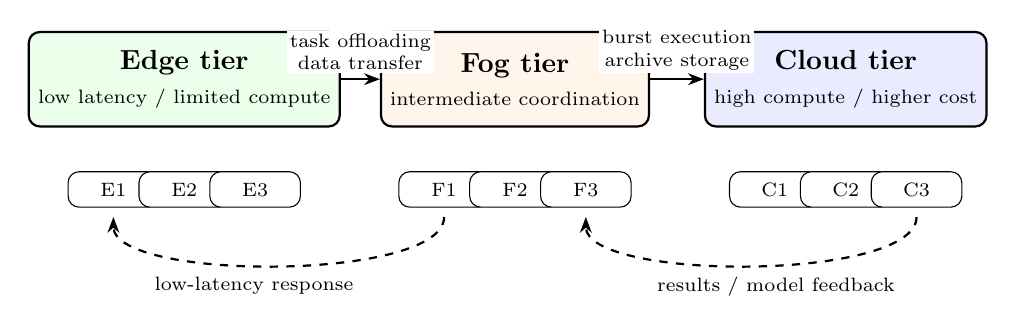
\begin{tikzpicture}[
  tier/.style={draw, rounded corners, thick, minimum width=3.4cm, minimum height=1.2cm, align=center, fill=#1!8},
  nbox/.style={draw, rounded corners, font=\scriptsize, inner sep=2pt, minimum width=1.15cm, minimum height=0.45cm, fill=white},
  link/.style={-{Stealth[length=2mm]}, thick}
]
  % Tier labels (top row)
  \node[tier=green]  (edge)  at (0,0)   {\textbf{Edge tier}\\\scriptsize low latency / limited compute};
  \node[tier=orange] (fog)   at (4.2,0) {\textbf{Fog tier}\\\scriptsize intermediate coordination};
  \node[tier=blue]   (cloud) at (8.4,0) {\textbf{Cloud tier}\\\scriptsize high compute / higher cost};

  % Node boxes (below tiers)
  \node[nbox] at (-0.9,-1.4) {E1};
  \node[nbox] at (0,   -1.4) {E2};
  \node[nbox] at (0.9, -1.4) {E3};

  \node[nbox] at (3.3,-1.4) {F1};
  \node[nbox] at (4.2,-1.4) {F2};
  \node[nbox] at (5.1,-1.4) {F3};

  \node[nbox] at (7.5,-1.4) {C1};
  \node[nbox] at (8.4,-1.4) {C2};
  \node[nbox] at (9.3,-1.4) {C3};

  % Forward arrows (between tiers, above node boxes)
  \draw[link] (edge.east)  -- node[midway, above=2pt, font=\scriptsize, align=center, fill=white, inner sep=1pt] {task offloading\\data transfer} (fog.west);
  \draw[link] (fog.east)   -- node[midway, above=2pt, font=\scriptsize, align=center, fill=white, inner sep=1pt] {burst execution\\archive storage} (cloud.west);

  % Feedback arrows (below node boxes)
  \draw[link, dashed] (9.3,-1.75) to[out=-90,in=-90, looseness=0.5]
    node[pos=0.45, below=3pt, font=\scriptsize, fill=white, inner sep=1pt] {results / model feedback}
    (5.1,-1.75);
  \draw[link, dashed] (3.3,-1.75) to[out=-90,in=-90, looseness=0.5]
    node[pos=0.55, below=3pt, font=\scriptsize, fill=white, inner sep=1pt] {low-latency response}
    (-0.9,-1.75);

\end{tikzpicture}
\caption{Simplified Edge/Fog/Cloud execution architecture used to motivate the scheduling model. The heterogeneous compute, bandwidth, and cost properties across tiers create the many-objective trade-offs optimized by ADARE and NSGA-III.}
\label{fig:edge_fog_cloud_arch}
\end{figure}

Figure~\ref{fig:edge_fog_cloud_arch} clarifies the systems setting: edge nodes favor low-latency execution, fog nodes provide coordination and intermediate capacity, and cloud nodes provide stronger compute at a different cost/bandwidth profile. This heterogeneity is the reason a static operator schedule can become suboptimal during search.

\subsection{Objective Vector}
ADARE and NSGA-III optimize the same four-objective minimization vector:
\begin{equation}
\min \; \mathbf{f}(x) = \left(f_{\mathrm{mk}}(x), f_{\mathrm{lat}}(x), f_{\mathrm{cost}}(x), f_{\mathrm{eng}}(x)\right),
\end{equation}
where:
\begin{itemize}
    \item $f_{\mathrm{mk}}$ is the workflow makespan (maximum task completion time);
    \item $f_{\mathrm{lat}}$ aggregates task completion delays relative to readiness times;
    \item $f_{\mathrm{cost}}$ accumulates compute-time-weighted processing cost across assigned nodes;
    \item $f_{\mathrm{eng}}$ accumulates compute-time-weighted working power as an execution energy proxy.
\end{itemize}
Let $C_i$, $R_i$, $I_i$, $\rho_{x_i}$, $c_{x_i}$, and $p^{\mathrm{wrk}}_{x_i}$ denote completion time, readiness time, task instructions, node processing rate, node cost, and node working power; cost and energy use execution-time weighting $I_i / \rho_{x_i}$.
The evaluator computes these metrics as:
\begin{equation}
\label{eq:objective_metrics}
\begin{aligned}
f_{\mathrm{mk}}(x) &= \max_{i \in V} C_i, \\
f_{\mathrm{lat}}(x) &= \sum_{i \in V} \left(C_i - R_i\right), \\
f_{\mathrm{cost}}(x) &= \sum_{i \in V} \left(\frac{I_i}{\rho_{x_i}}\right) c_{x_i}, \\
f_{\mathrm{eng}}(x) &= \sum_{i \in V} \left(\frac{I_i}{\rho_{x_i}}\right) p^{\mathrm{wrk}}_{x_i}.
\end{aligned}
\end{equation}

This reflects the core edge/fog/cloud tension: faster assignments can reduce completion time while increasing cost or energy, so we target a diverse Pareto set rather than a single operating point.

\subsection{Evaluation Targets and Quality Indicators}
In addition to objective values, we evaluate search quality using hypervolume (HV), inverted generational distance (IGD), spacing, additive epsilon, and coverage. No single indicator was reliable enough on its own in our runs, so we keep this set to read front quality from complementary angles (dominance coverage, convergence to a reference front, and spread regularity). For ADARE, that distinction matters: the controller is meant to improve search behavior over time, not just one objective extreme.

% Experimental intuition added
With the objective vector and evaluation targets fixed, we now describe how the search loop uses this feedback online.

\section{ADARE Methodology: Learning-Guided Adaptive Control}
\subsection{Design Overview}
ADARE keeps the many-objective selection backbone of NSGA-III and replaces fixed operator control with an online adaptive layer. Figure~\ref{fig:adare_structure} summarizes this organization.

\begin{figure}[t]
\centering
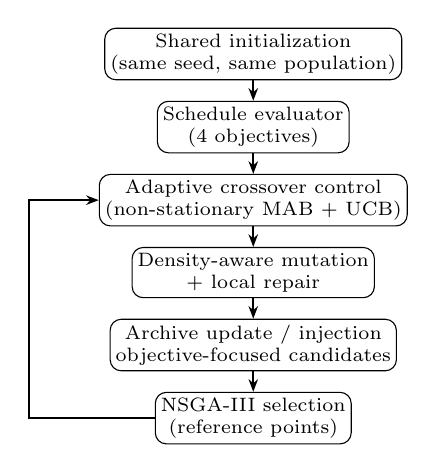
\begin{tikzpicture}[
node distance=2.6mm,
box/.style={draw, rounded corners, align=center, font=\scriptsize, inner sep=2pt},
arr/.style={-{Stealth[length=1.6mm]}, thick}
]
\node[box] (init) {Shared initialization\\(same seed, same population)};
\node[box, below=of init] (eval) {Schedule evaluator\\(4 objectives)};
\node[box, below=of eval] (cross) {Adaptive crossover control\\(non-stationary MAB + UCB)};
\node[box, below=of cross] (mut) {Density-aware mutation\\+ local repair};
\node[box, below=of mut] (arch) {Archive update / injection\\objective-focused candidates};
\node[box, below=of arch] (sel) {NSGA-III selection\\(reference points)};
\draw[arr] (init) -- (eval);
\draw[arr] (eval) -- (cross);
\draw[arr] (cross) -- (mut);
\draw[arr] (mut) -- (arch);
\draw[arr] (arch) -- (sel);
\draw[arr] (sel.west) -- ++(-1.6,0) |- (cross.west);
\end{tikzpicture}
\caption{ADARE as a learning-guided control layer embedded in the NSGA-III search loop.}
\label{fig:adare_structure}
\end{figure}

% Experimental intuition added
We kept this architecture on purpose: replacing the full optimizer with a monolithic learner would blur attribution in paired comparisons. Instead, we adapt operator choice and diversity recovery while keeping NSGA-III selection unchanged, which preserves interpretability and a practical runtime profile.

\subsection{Learning Formalization: Non-stationary MAB for Operator Control}
\label{sec:mab}
At each generation, ADARE selects a crossover operator from a small portfolio (one-point, two-point, and uniform variants). We model this choice as a multi-armed bandit (MAB) problem. The formulation is intentionally local: a compact controller is easier to instrument, debug, and compare fairly than a higher-capacity policy module in this artifact setting. The reward distribution is non-stationary because population diversity, front geometry, and feasibility structure evolve during search \cite{auer2002ucb,besbes2014nonstationary}, which makes static crossover probabilities a poor fit for heterogeneous workflow scheduling.

Let $Q_k$ be the current quality estimate for operator $k$, and $N_k$ its usage count. At decision step $t$, ADARE chooses the operator with the UCB rule:
\begin{equation}
\label{eq:ucb}
a_t = \arg\max_k \left( Q_k + \sqrt{\frac{2 \ln t}{N_k + 1}} \right).
\end{equation}
The second term maintains exploration, while the first term exploits operators with strong recent rewards.

\paragraph{Reward definition.}
We define the reward as a scalar Pareto-quality improvement proxy computed on the parent-offspring comparison:
\begin{equation}
\label{eq:reward}
r_t = \phi\!\left(\min\{p_1,p_2\}\right) - \phi\!\left(\min\{c_1,c_2\}\right),
\end{equation}
where $\phi(\cdot)$ is a log-scaled scalarization proxy (smaller is better). We retained this proxy after a few implementation attempts because front-level indicators at every mating event made operator-level attribution both expensive and noisy. A positive reward indicates that the selected operator produced better offspring according to the proxy. ADARE updates the selected operator value by exponential smoothing:
\begin{equation}
Q_k \leftarrow (1-\alpha)Q_k + \alpha r_t.
\end{equation}
This keeps operator control in an online-learning regime, while the update itself remains cheap enough for clean overhead measurements. Algorithm~\ref{alg:ucb_control} gives the exact decision/update sequence used per mating event.

\begin{algorithm}[H]
\caption{ADARE UCB-Based Crossover Control}
\label{alg:ucb_control}
\small
\begin{algorithmic}[1]
\Require Parent pair $(p_1,p_2)$, scores $Q$, usage counts $N$, step $t$
\State Select operator index $k$ with Eq.~\eqref{eq:ucb}
\State Apply crossover operator $k$ to obtain $(c_1,c_2)$
\State Compute reward $r_t$ with Eq.~\eqref{eq:reward}
\State Update $Q_k \leftarrow (1-\alpha)Q_k + \alpha r_t$ and $N_k \leftarrow N_k + 1$
\State \Return $(c_1,c_2)$
\end{algorithmic}
\end{algorithm}

\subsection{Density-Aware Mutation and Local Repair}
ADARE's mutation layer adapts perturbation effort using generation progress and population diversity. When diversity collapses, mutation pressure increases; when diversity is healthy, mutation stays conservative. A heuristic task-node ranking (processing speed, bandwidth, cost, power) biases part of the mutations toward plausible assignments, with a random fallback to avoid early over-commitment. Algorithm~\ref{alg:density_mutation} summarizes the mutation and repair sequence used in each generation.

\begin{algorithm}[H]
\caption{Density-Aware Mutation with Heuristic Guidance}
\label{alg:density_mutation}
\small
\begin{algorithmic}[1]
\Require Individual $x$, diversity score $d$, generation $g$, task-node rankings $\mathcal{R}$
\State Compute mutation budget $B \gets f(g,d)$ (larger when diversity decreases)
\For{$b = 1$ to $B$}
    \State Sample a task index $i$
    \State Set $x_i$ using heuristic-ranked nodes or a random fallback
\EndFor
\State Apply a low-probability gene-level mutation pass
\State Optionally perform a small greedy local repair
\State \Return mutated individual $x$
\end{algorithmic}
\end{algorithm}

\subsection{Archive Guidance and Objective-Focused Final Candidate Pool}
ADARE maintains a bounded archive of strong non-dominated or high-value candidates. During evolution, archive injection is rate-limited to guide search without collapsing diversity. At the end of the run, ADARE separates two roles: (i) the final non-dominated population for Pareto-quality metrics (HV, IGD, spacing, epsilon, coverage), and (ii) an objective-focused pool augmented with archive and targeted candidates for best-objective reporting (e.g., makespan or latency extremes). Algorithm~\ref{alg:archive_pool} details this construction.

\begin{algorithm}[H]
\caption{Archive-Guided Final Objective Pool Construction}
\label{alg:archive_pool}
\small
\begin{algorithmic}[1]
\Require Final population $P$, archive $A$, targeted candidate set $K$
\State $P^{\mathrm{obj}} \gets P \cup A$
\ForAll{$k \in K$}
    \If{$k$ improves at least one tracked objective extreme}
        \State Insert $k$ into $P^{\mathrm{obj}}$
    \EndIf
\EndFor
\State \Return $P$ for Pareto-quality metrics and $P^{\mathrm{obj}}$ for objective-best metrics
\end{algorithmic}
\end{algorithm}

\subsection{Complexity and Measured Control Overhead}
The schedule evaluator dominates runtime. For population size $P$, generation count $G$, task count $|V|$, and average dependency-processing factor $\bar d$, evaluation cost is approximately
\begin{equation}
\mathcal{O}(G \cdot P \cdot |V| \cdot \bar d).
\end{equation}
The UCB controller adds constant-time operations per operator decision (mean update, counter update, logarithm, square root), while archive operations are bounded on a small structure. In this artifact, the schedule evaluator still dominates wall-clock time for realistic workflow sizes.

% Experimental intuition added
To verify this empirically, we instrumented UCB selection and update, together with archive routines, on 15 representative runs (5 seeds per benchmark). The measured upper-bound control ratio is \textbf{5.17\% on average} (maximum \textbf{5.34\%}) of total ADARE runtime. The instrumentation was intentionally conservative at Python level, so the ratio should be read as an upper bound rather than an exact decomposition of every micro-operation. It nevertheless supports the intended near-5\% overhead target while preserving measurable quality gains.

\section{Experimental Protocol and Results}
\subsection{Artifact, Local Execution Context, and Hardware Configuration}
All experiments were executed locally using the code in the current ADARE artifact (no cluster). We report the host details from system diagnostics because runtime differences at this scale are sensitive to workstation-level CPU and memory behavior.

\begin{table}[t]
\caption{Local Host Machine (from system diagnostics)}
\label{tab:hardware}
\centering
\small
\begin{tabularx}{\textwidth}{@{}l X@{}}
\toprule
Item & Specification \\
\midrule
System model & ASUS TUF Gaming A15 FA506NF\_FA506NF (ASUSTeK COMPUTER INC.) \\
Host OS & Windows 11 Home 64-bit, Build 26200 (dxdiag timestamp: 2025-12-18) \\
CPU & AMD Ryzen 5 7535HS with Radeon Graphics, 12 logical CPUs, \SI{3.3}{GHz} nominal \\
RAM & \SI{16}{GB} installed (\SI{15.69}{GB} available in dxdiag) \\
GPU(s) & AMD Radeon(TM) Graphics + NVIDIA GeForce RTX 2050 (\SI{3.964}{GB} dedicated reported) \\
Display / mode & 1920$\times$1080; host reports 144~Hz internal panel and 75~Hz external display \\
\bottomrule
\end{tabularx}
\end{table}

% Author reasoning clarification
Table~\ref{tab:hardware} is operationally important because runtime gains in Python MOEAs depend on CPU generation and memory behavior. This became especially relevant when some longer runs were split into batches for execution stability. The local software stack used for the experiments is Python 3.13.1 with \texttt{numpy 2.2.5}, \texttt{matplotlib 3.10.8}, \texttt{deap 1.4}, \texttt{scipy 1.16.3}, and \texttt{pymoo 0.6.1.6}.

\subsection{Benchmarks and Heterogeneous Resource Configuration}
We evaluate three workflow instances commonly used in scientific workflow scheduling: \texttt{Montage\_25}, \texttt{CyberShake\_30}, and \texttt{Epigenomics\_24}. These workflow families are available through public repositories used in the Pegasus and WfCommons ecosystems \cite{coleman2021wfcommons}.

The heterogeneous resource model is defined in the experiment configuration. Table~\ref{tab:envjson} reproduces the exact tier-level parameters used in the artifact.

\begin{table}[t]
\caption{Resource Configuration Used in Experiments}
\label{tab:envjson}
\centering
\small
\begin{tabular}{@{}lrrrrrr@{}}
\toprule
Tier & Devices & Proc. rate & Cost & Idle P. & Work P. & Up/Down BW \\
\midrule
Edge & 5 & 1000 & 0.02 & 30 & 700 & 20480 / 20480 \\
Fog & 5 & 1300 & 0.48 & 30 & 700 & 10000 / 10000 \\
Cloud & 5 & 1600 & 0.96 & 1332 & 1648 & 100 / 10000 \\
\bottomrule
\end{tabular}
\end{table}

This table creates the optimization tension used throughout the study. In early debugging runs, it was easy to over-focus on cloud processing rate alone; the bandwidth asymmetry and cost/power gradients explain why that intuition is often wrong.

\subsection{Fairness Protocol, Metrics, and Statistical Testing}
ADARE and NSGA-III share the same evaluation function, generation budget, and initial population at each paired run. The artifact generates a shared initial population from the same seed before instantiating both algorithms, which enforces a fair comparison baseline.

% Author reasoning clarification
We report \textbf{20 paired runs per benchmark}. In our runs on the workstation, benchmarks are executed sequentially (one workflow family at a time) to avoid runtime perturbations from concurrent processes. The statistical design is unchanged: paired 20-run comparisons.

Reported outputs include: (i) Pareto-quality metrics (HV, IGD, spacing, epsilon, coverage), (ii) runtime, and (iii) best objective values for makespan, latency, cost, and energy. For statistical validation, we use the paired Wilcoxon signed-rank test and Cliff's delta effect size \cite{wilcoxon1945,cliff1993}.

\subsection{Main Results: 20-Run Paired Comparison (ADARE vs NSGA-III)}
Table~\ref{tab:main20} summarizes the main comparative outcomes (means over 20 paired runs). NSGA-III means are shown in parentheses for direct readability.

\begin{table}[t]
\caption{20-Run Summary (ADARE vs NSGA-III, means; NSGA-III in parentheses)}
\label{tab:main20}
\centering
\small
\begin{tabular}{@{}lccccc@{}}
\toprule
Benchmark & HV & IGD & $\Delta$ Mk. (\%) & $\Delta$ Lat. (\%) & $\Delta t$ (\%) \\
\midrule
Montage\_25 & 0.9493 (0.9232) & 0.0600 (0.0624) & 19.01 & 11.77 & 4.89 \\
CyberShake\_30 & 0.9645 (0.9303) & 0.0633 (0.0718) & 5.17 & 8.01 & 7.47 \\
Epigenomics\_24 & 1.0453 (1.0337) & 0.0342 (0.0414) & 1.18 & 4.34 & 4.13 \\
\bottomrule
\end{tabular}
\end{table}

ADARE improves HV on all three workflows and improves makespan/latency extremes in every case. In the final 20-run configuration, IGD also improves on all three workflows. This is useful because it means the stronger extremes and spread do not come at the expense of distance-to-reference quality in the reported protocol.

\begin{table}[t]
\caption{Statistical Evidence (20 Paired Runs): Wilcoxon $p$ and Cliff's $\delta$}
\label{tab:stats20}
\centering
\scriptsize
\begin{tabular}{@{}l l c c@{}}
\toprule
Benchmark & Metric & Wilcoxon $p$ & Cliff's $\delta$ \\
\midrule
\multirow{3}{*}{Montage\_25}
& HV & $1.05\times10^{-4}$ & 0.645 (large) \\
& Coverage & $1.33\times10^{-2}$ & 0.440 (medium) \\
& Runtime & $6.04\times10^{-3}$ & 0.725 (large) \\
\midrule
\multirow{3}{*}{CyberShake\_30}
& HV & $1.91\times10^{-6}$ & 0.980 (large) \\
& IGD & $9.54\times10^{-7}$ & 0.940 (large) \\
& Runtime & $1.97\times10^{-4}$ & 0.760 (large) \\
\midrule
\multirow{3}{*}{Epigenomics\_24}
& HV & $9.54\times10^{-7}$ & 0.960 (large) \\
& Spacing & $9.54\times10^{-7}$ & 0.965 (large) \\
& Runtime & $2.66\times10^{-2}$ & 0.325 (small) \\
\bottomrule
\end{tabular}
\end{table}

% Discussion refinement
Table~\ref{tab:stats20} confirms that the quality gains are not only visual. HV improvements are significant on all three workflows, and the selected runtime comparisons are also significant in this final protocol. Epigenomics nevertheless remains the benchmark where runtime gains are the smallest in effect size (small Cliff's $\delta$), even when the direction is favorable.

In our runs across the three benchmarks, ADARE wins \textbf{18/18} quality comparisons (including runtime) and \textbf{15/15} core-quality comparisons (excluding runtime). Average gains are \textbf{26.80\%} in core quality, \textbf{10.70\%} in best-objective metrics, and \textbf{5.50\%} in runtime.

\subsection{Ablation Protocol (V1--V5) and Artifact-Ready Variant Definition}
To isolate module effects in our runs, we keep the same paired-run fairness constraints and grow the ablation step by step. We start with \textbf{V1} (NSGA-III baseline), then add UCB crossover control in \textbf{V2}, density-aware mutation in \textbf{V3}, partial archive injection/final-pool guidance in \textbf{V4}, and full ADARE in \textbf{V5}.

\begin{table}[t]
\caption{Ablation Variants (Design Matrix for the 20-Run Protocol)}
\label{tab:ablation_design}
\centering
\small
\begin{tabular}{@{}lccc@{}}
\toprule
Variant & UCB crossover & Density-aware mutation & Archive/objective pool \\
\midrule
V1 (NSGA-III) & No & No & No \\
V2 & Yes & No & No \\
V3 & Yes & Yes & No \\
V4 & Yes & Yes & Yes (partial) \\
V5 (ADARE full) & Yes & Yes & Yes (full config) \\
\bottomrule
\end{tabular}
\end{table}

This paper reports the completed 20-run ADARE-vs-NSGA-III comparison and provides the V1--V5 ablation protocol and variant mapping for the extended artifact. Methodologically, the gains are better interpreted as the interaction of several control components than as the effect of a single heuristic switch.

\subsection{Qualitative Pareto and Convergence Analysis}
We inspect representative Pareto projections and convergence traces next because the tables alone do not show \emph{how} the search behavior changes.

\begin{figure}[t]
\centering
\begin{minipage}[t]{0.48\textwidth}
\centering
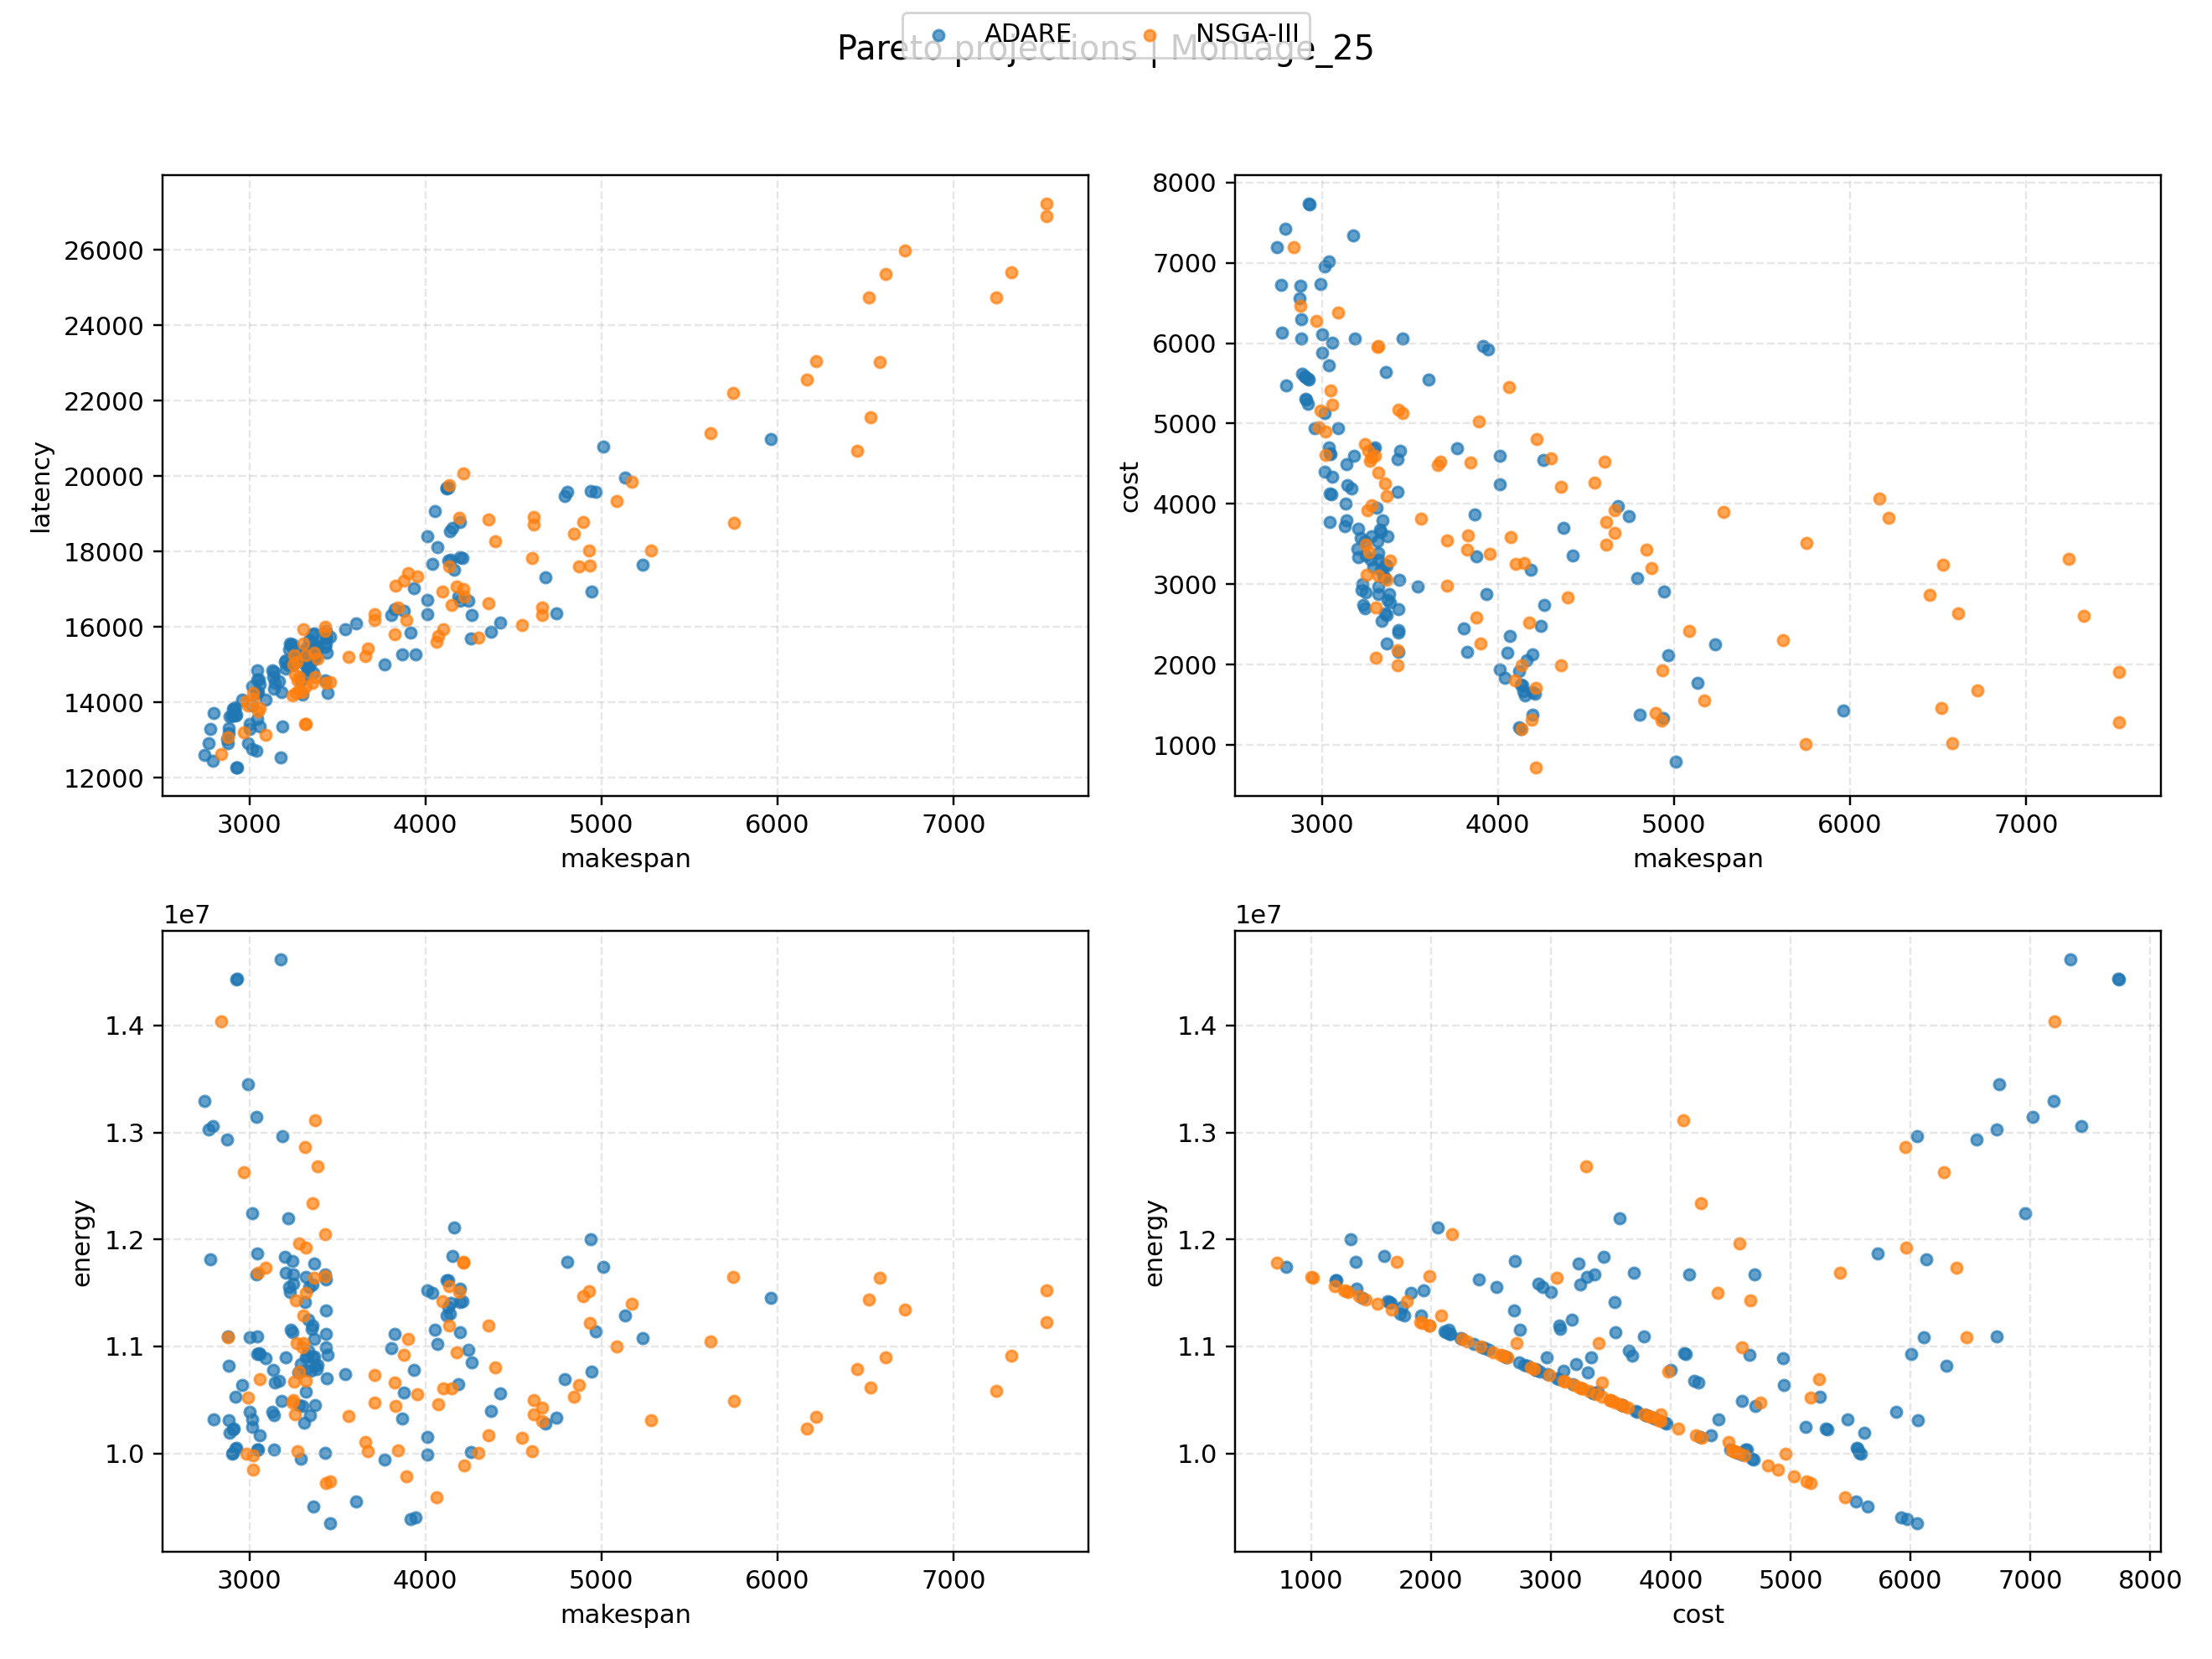
\includegraphics[width=\linewidth]{pareto_test_montage25.png}\\[-0.5ex]
\scriptsize (a) Montage\_25
\end{minipage}\hfill
\begin{minipage}[t]{0.48\textwidth}
\centering
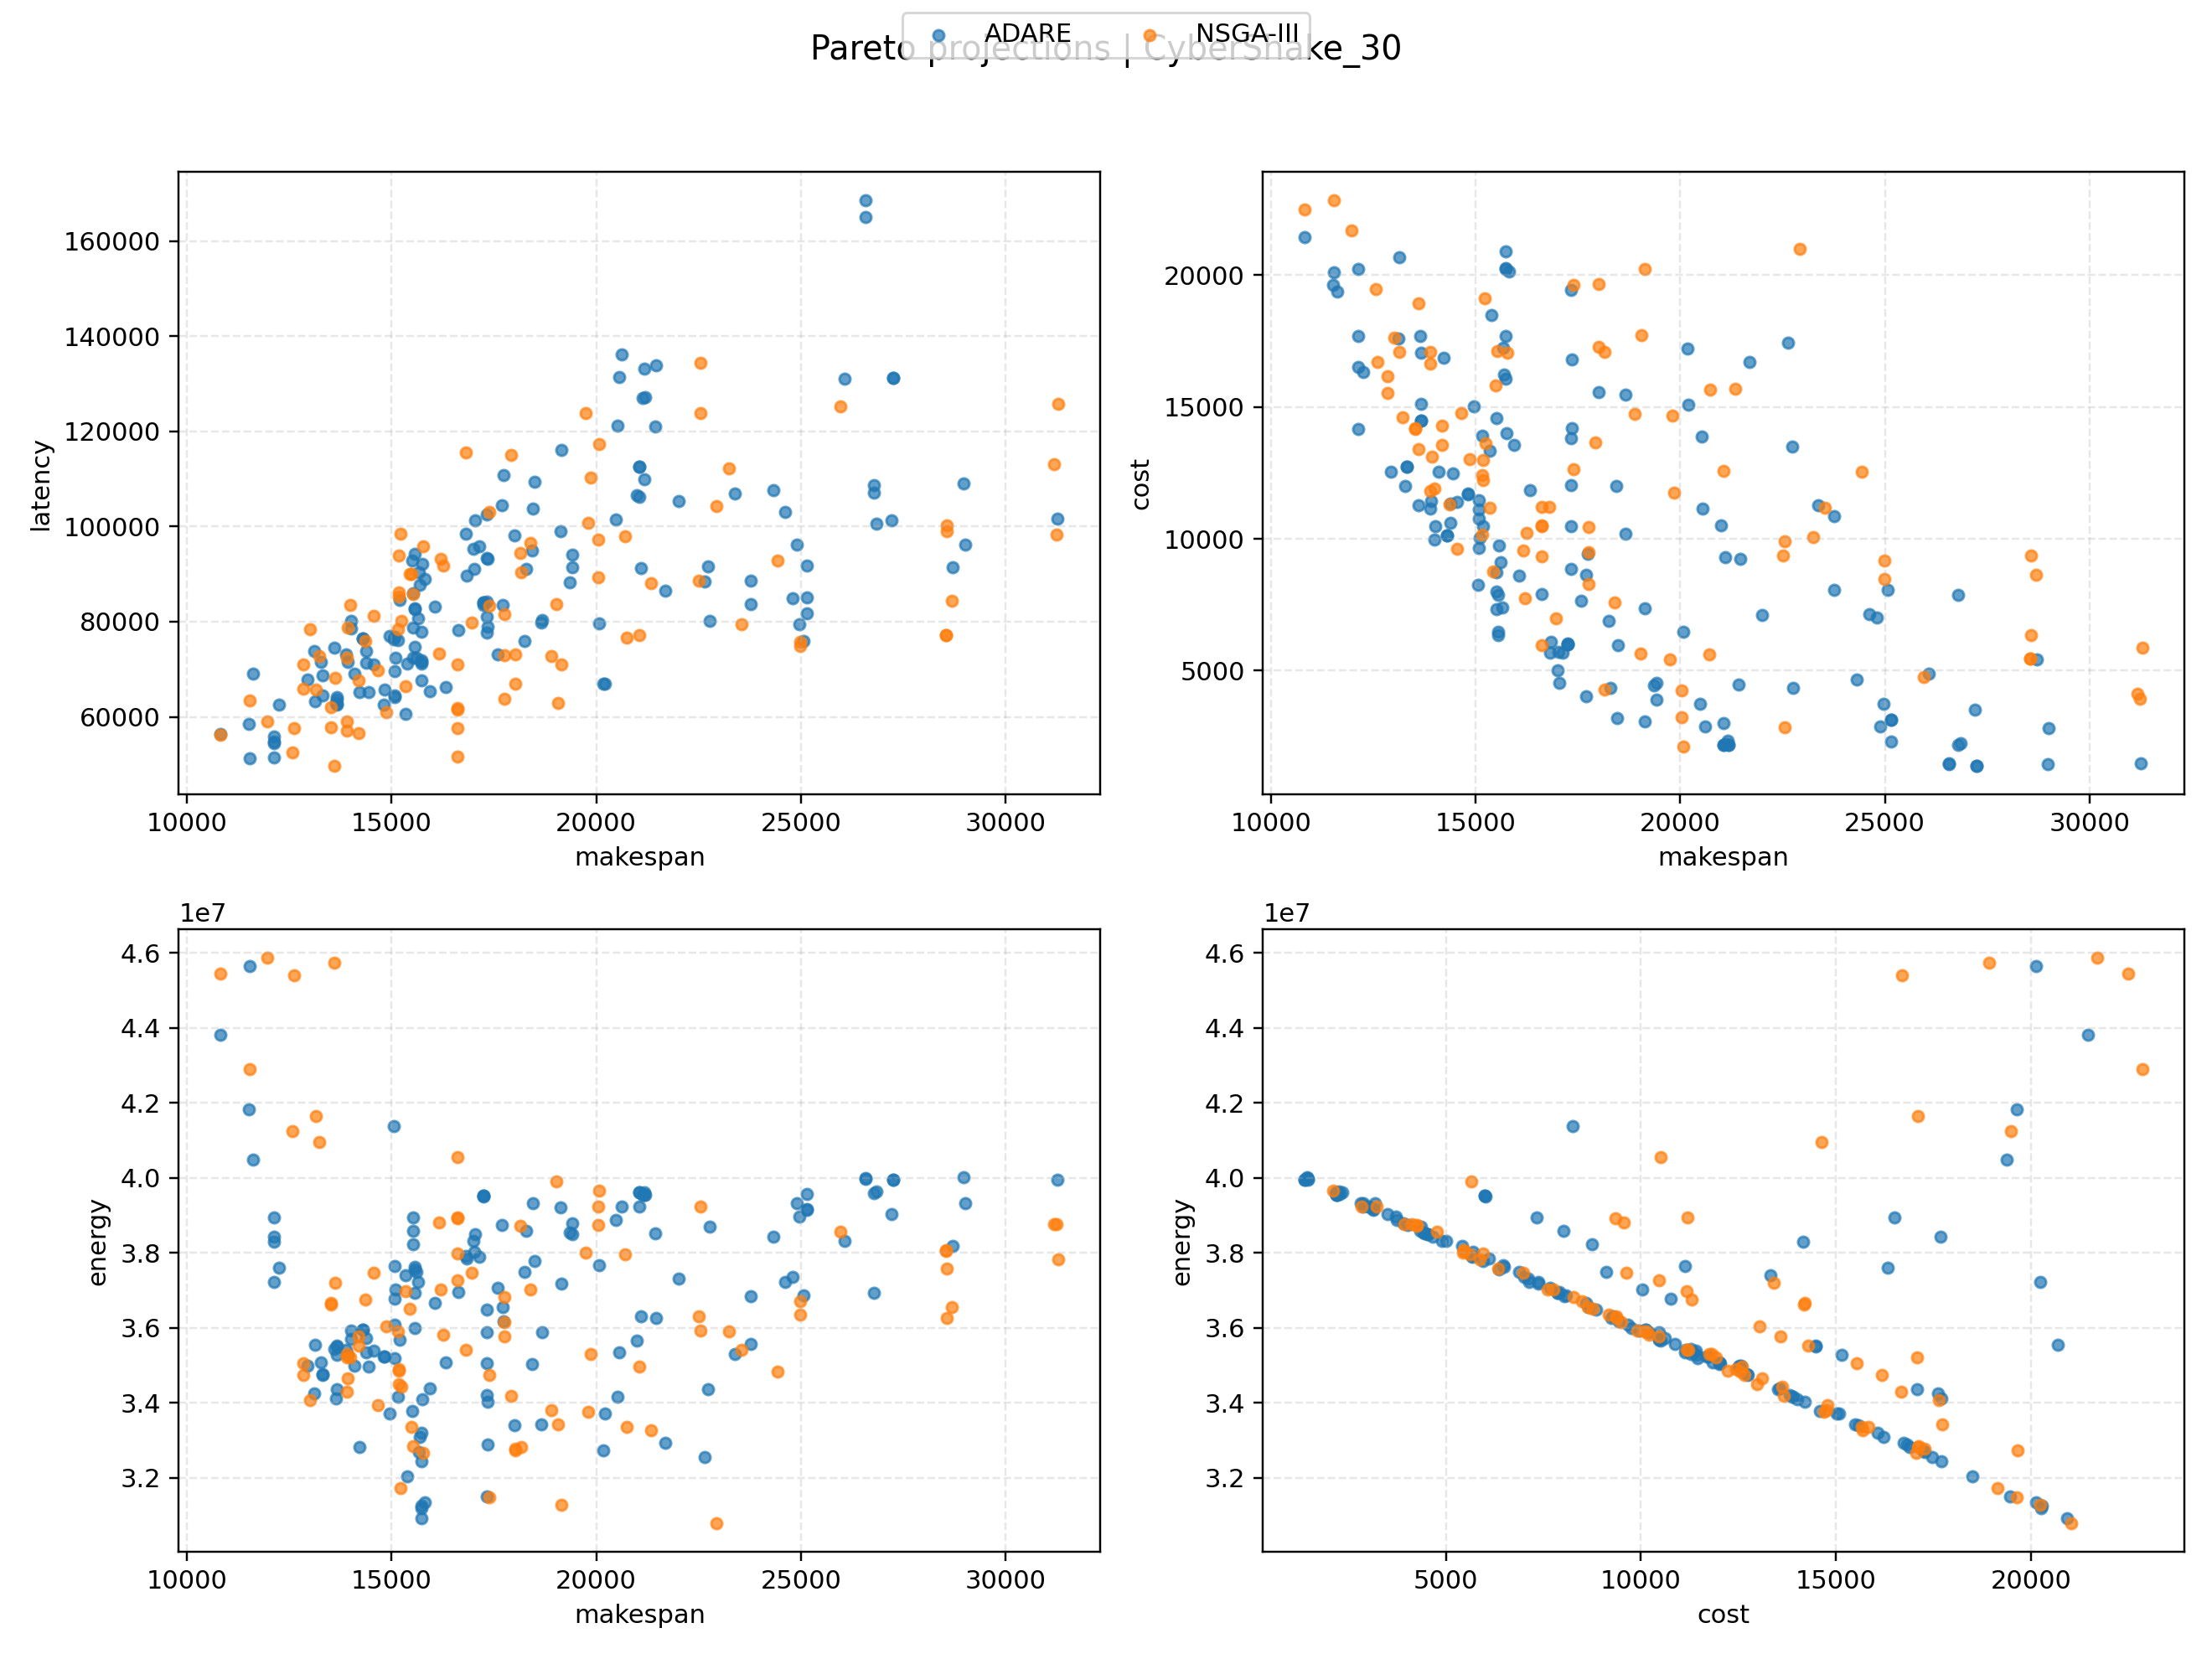
\includegraphics[width=\linewidth]{pareto_test_cybershake30.png}\\[-0.5ex]
\scriptsize (b) CyberShake\_30
\end{minipage}

\vspace{0.6ex}

\begin{minipage}[t]{0.68\textwidth}
\centering
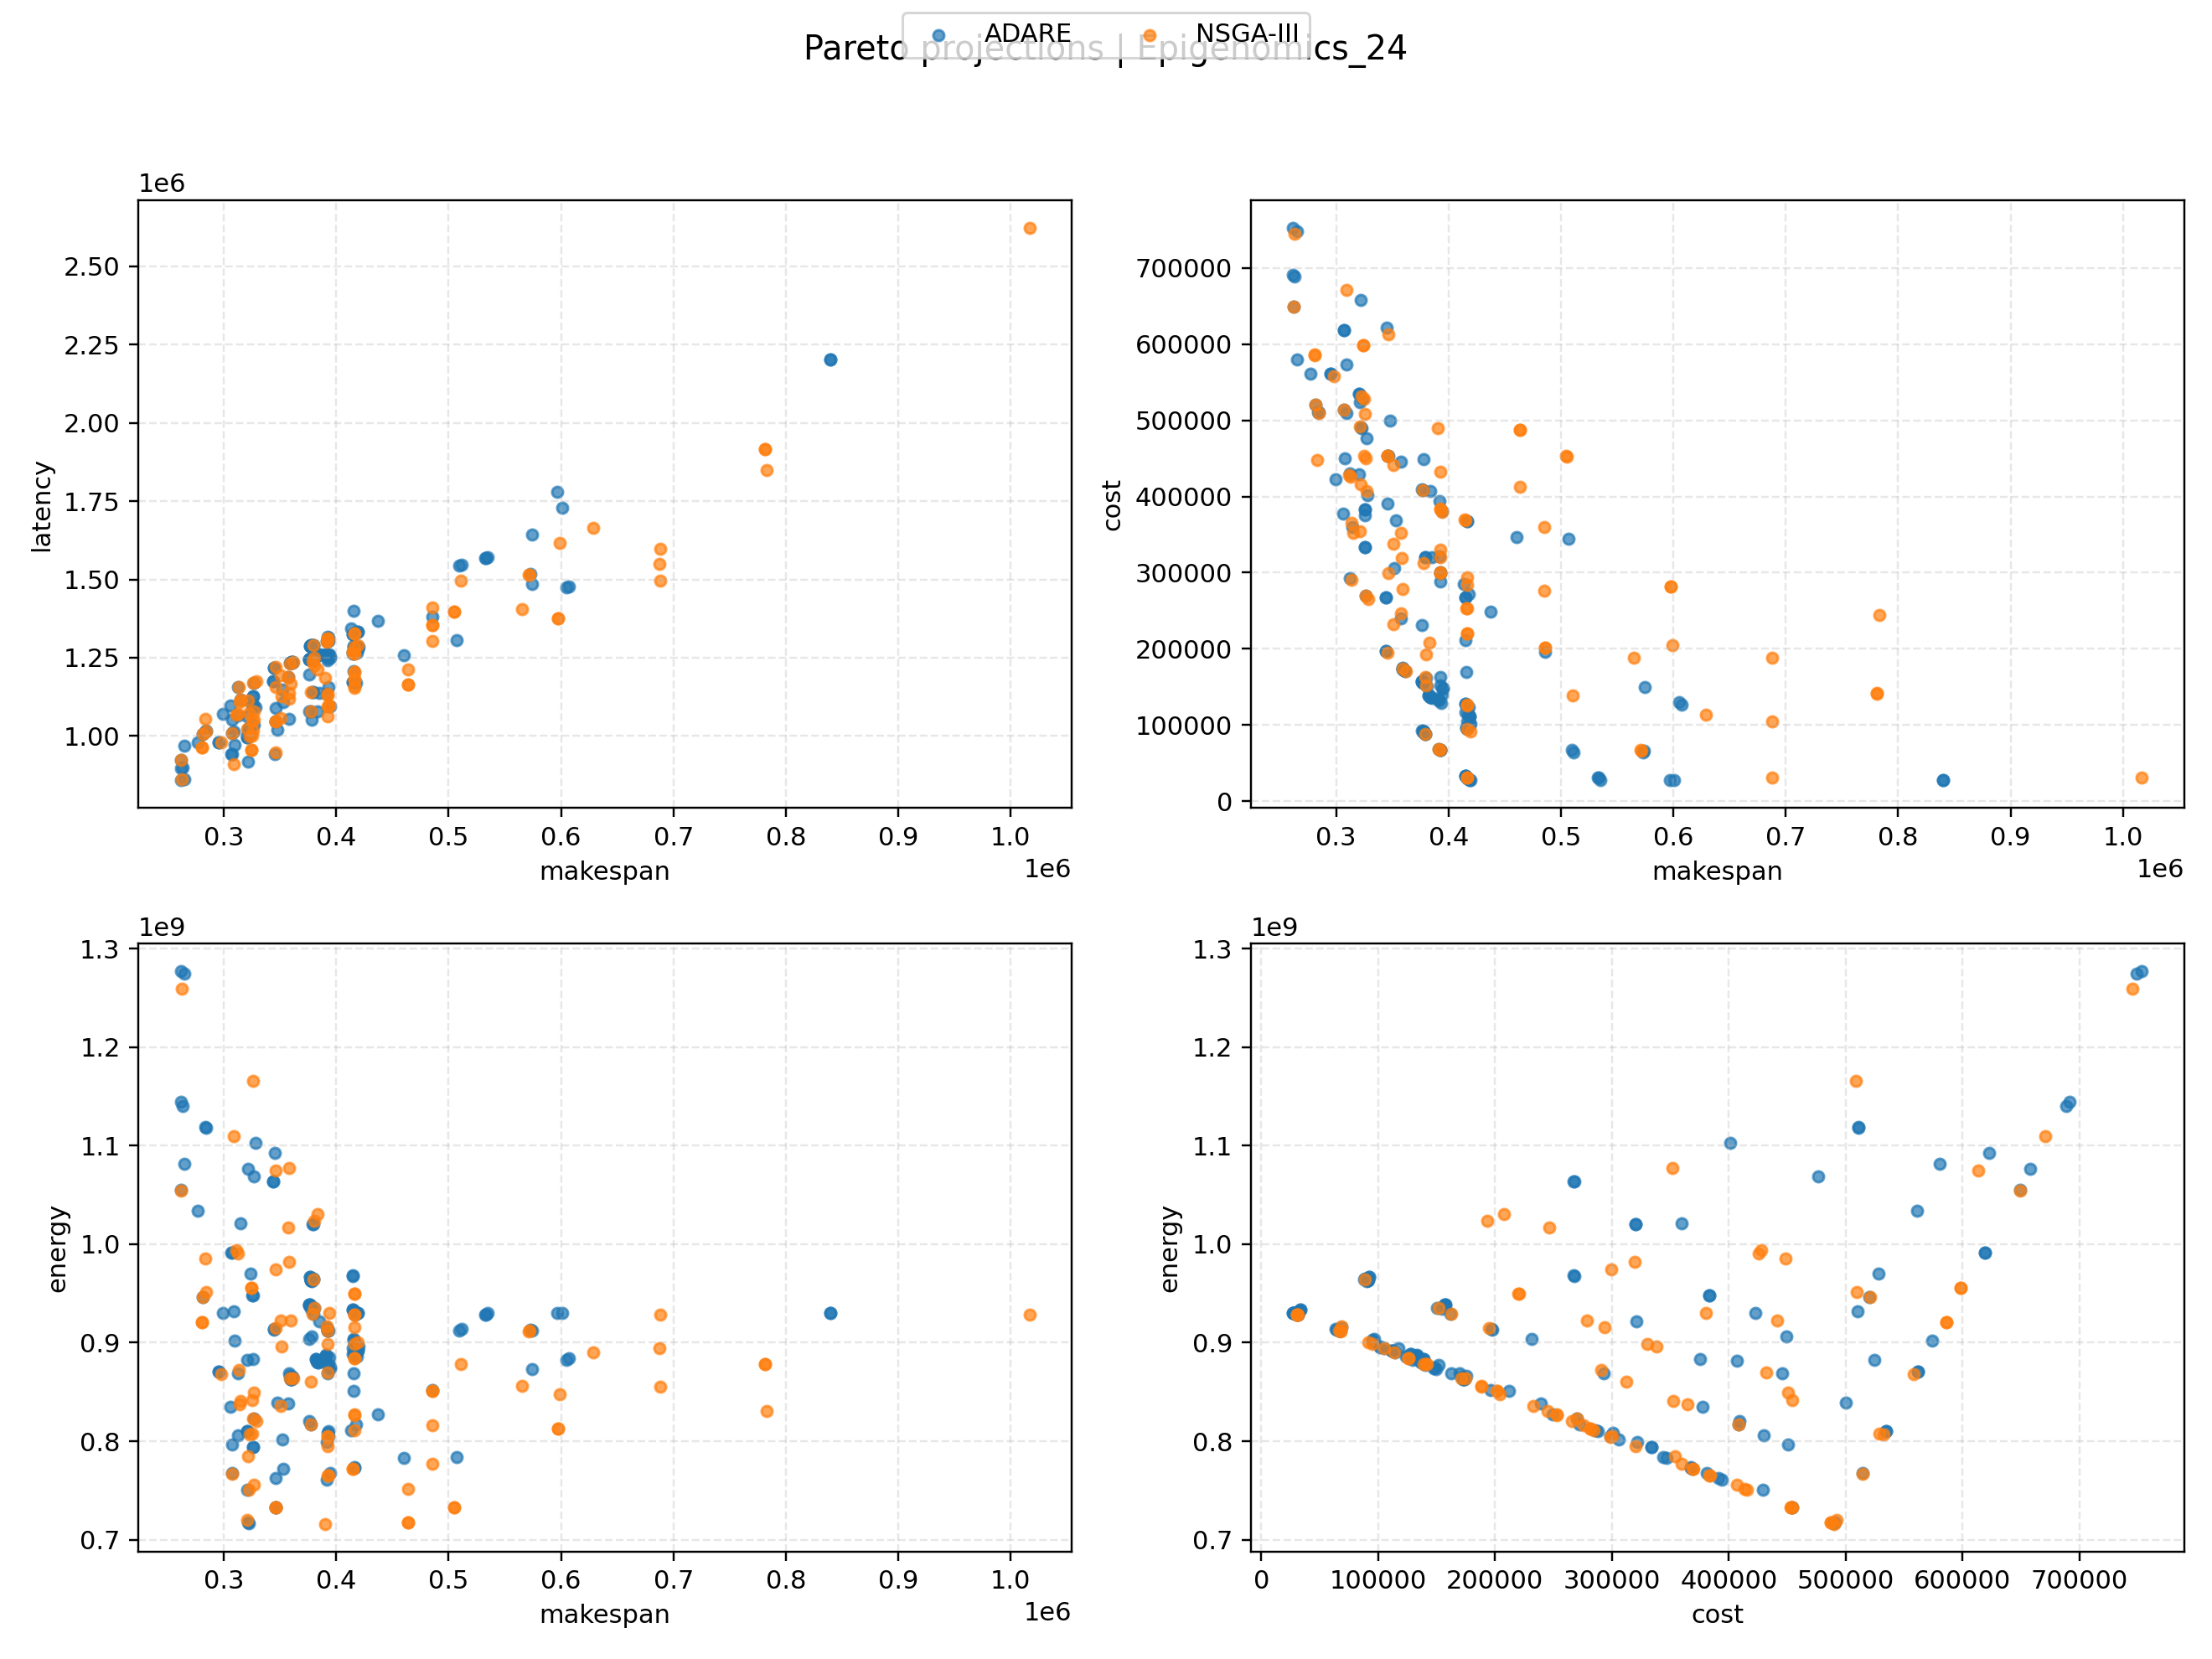
\includegraphics[width=\linewidth]{pareto_test_epigenomics24.png}\\[-0.5ex]
\scriptsize (c) Epigenomics\_24
\end{minipage}
\caption{Representative Pareto projections (ADARE vs NSGA-III) across the three workflow families. Larger panels are used here for readability of the projected fronts and dominance regions.}
\label{fig:pareto_all}
\end{figure}

Figure~\ref{fig:pareto_all} is consistent with the quantitative results: ADARE extends favorable regions on Montage, broadens coverage on CyberShake, and improves spread on Epigenomics while preserving strong objective extremes. The Epigenomics plots are particularly useful here because the visual spread improvement is easier to see than the runtime effect.

\begin{figure}[t]
\centering
\begin{minipage}[t]{0.48\textwidth}
\centering
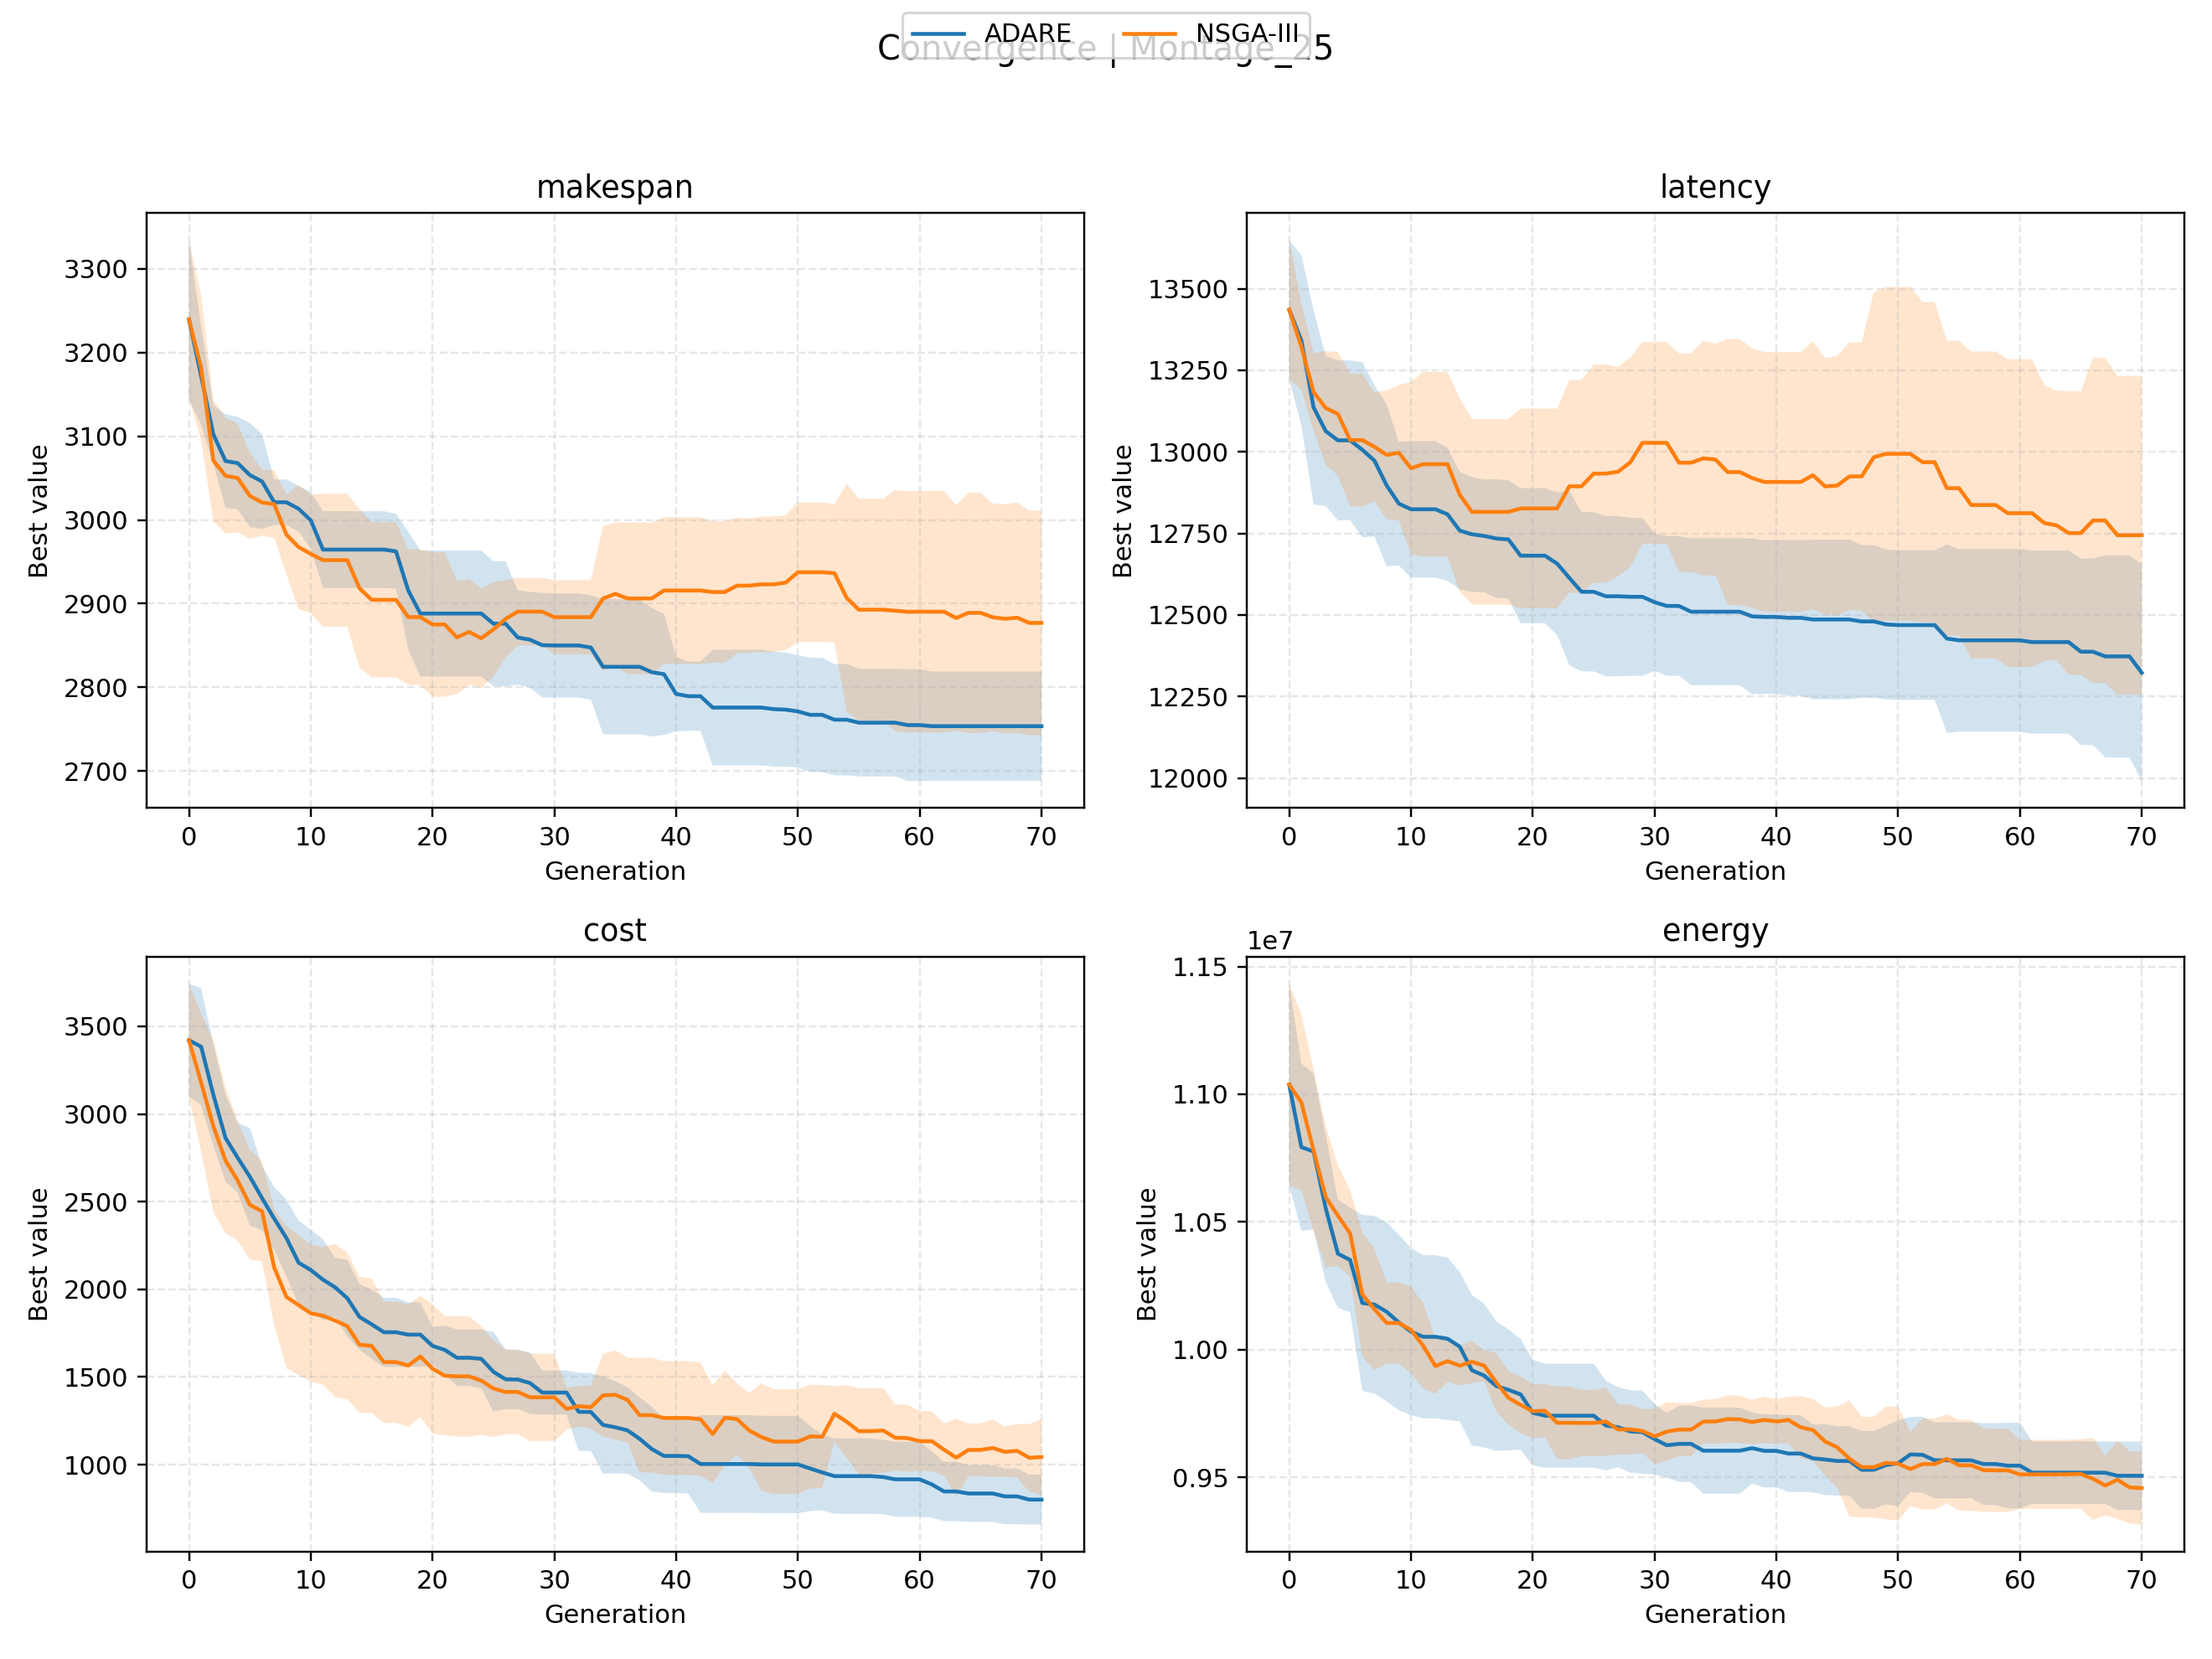
\includegraphics[width=\linewidth]{convergence_test_montage25.png}\\[-0.5ex]
\scriptsize (a) Montage\_25
\end{minipage}\hfill
\begin{minipage}[t]{0.48\textwidth}
\centering
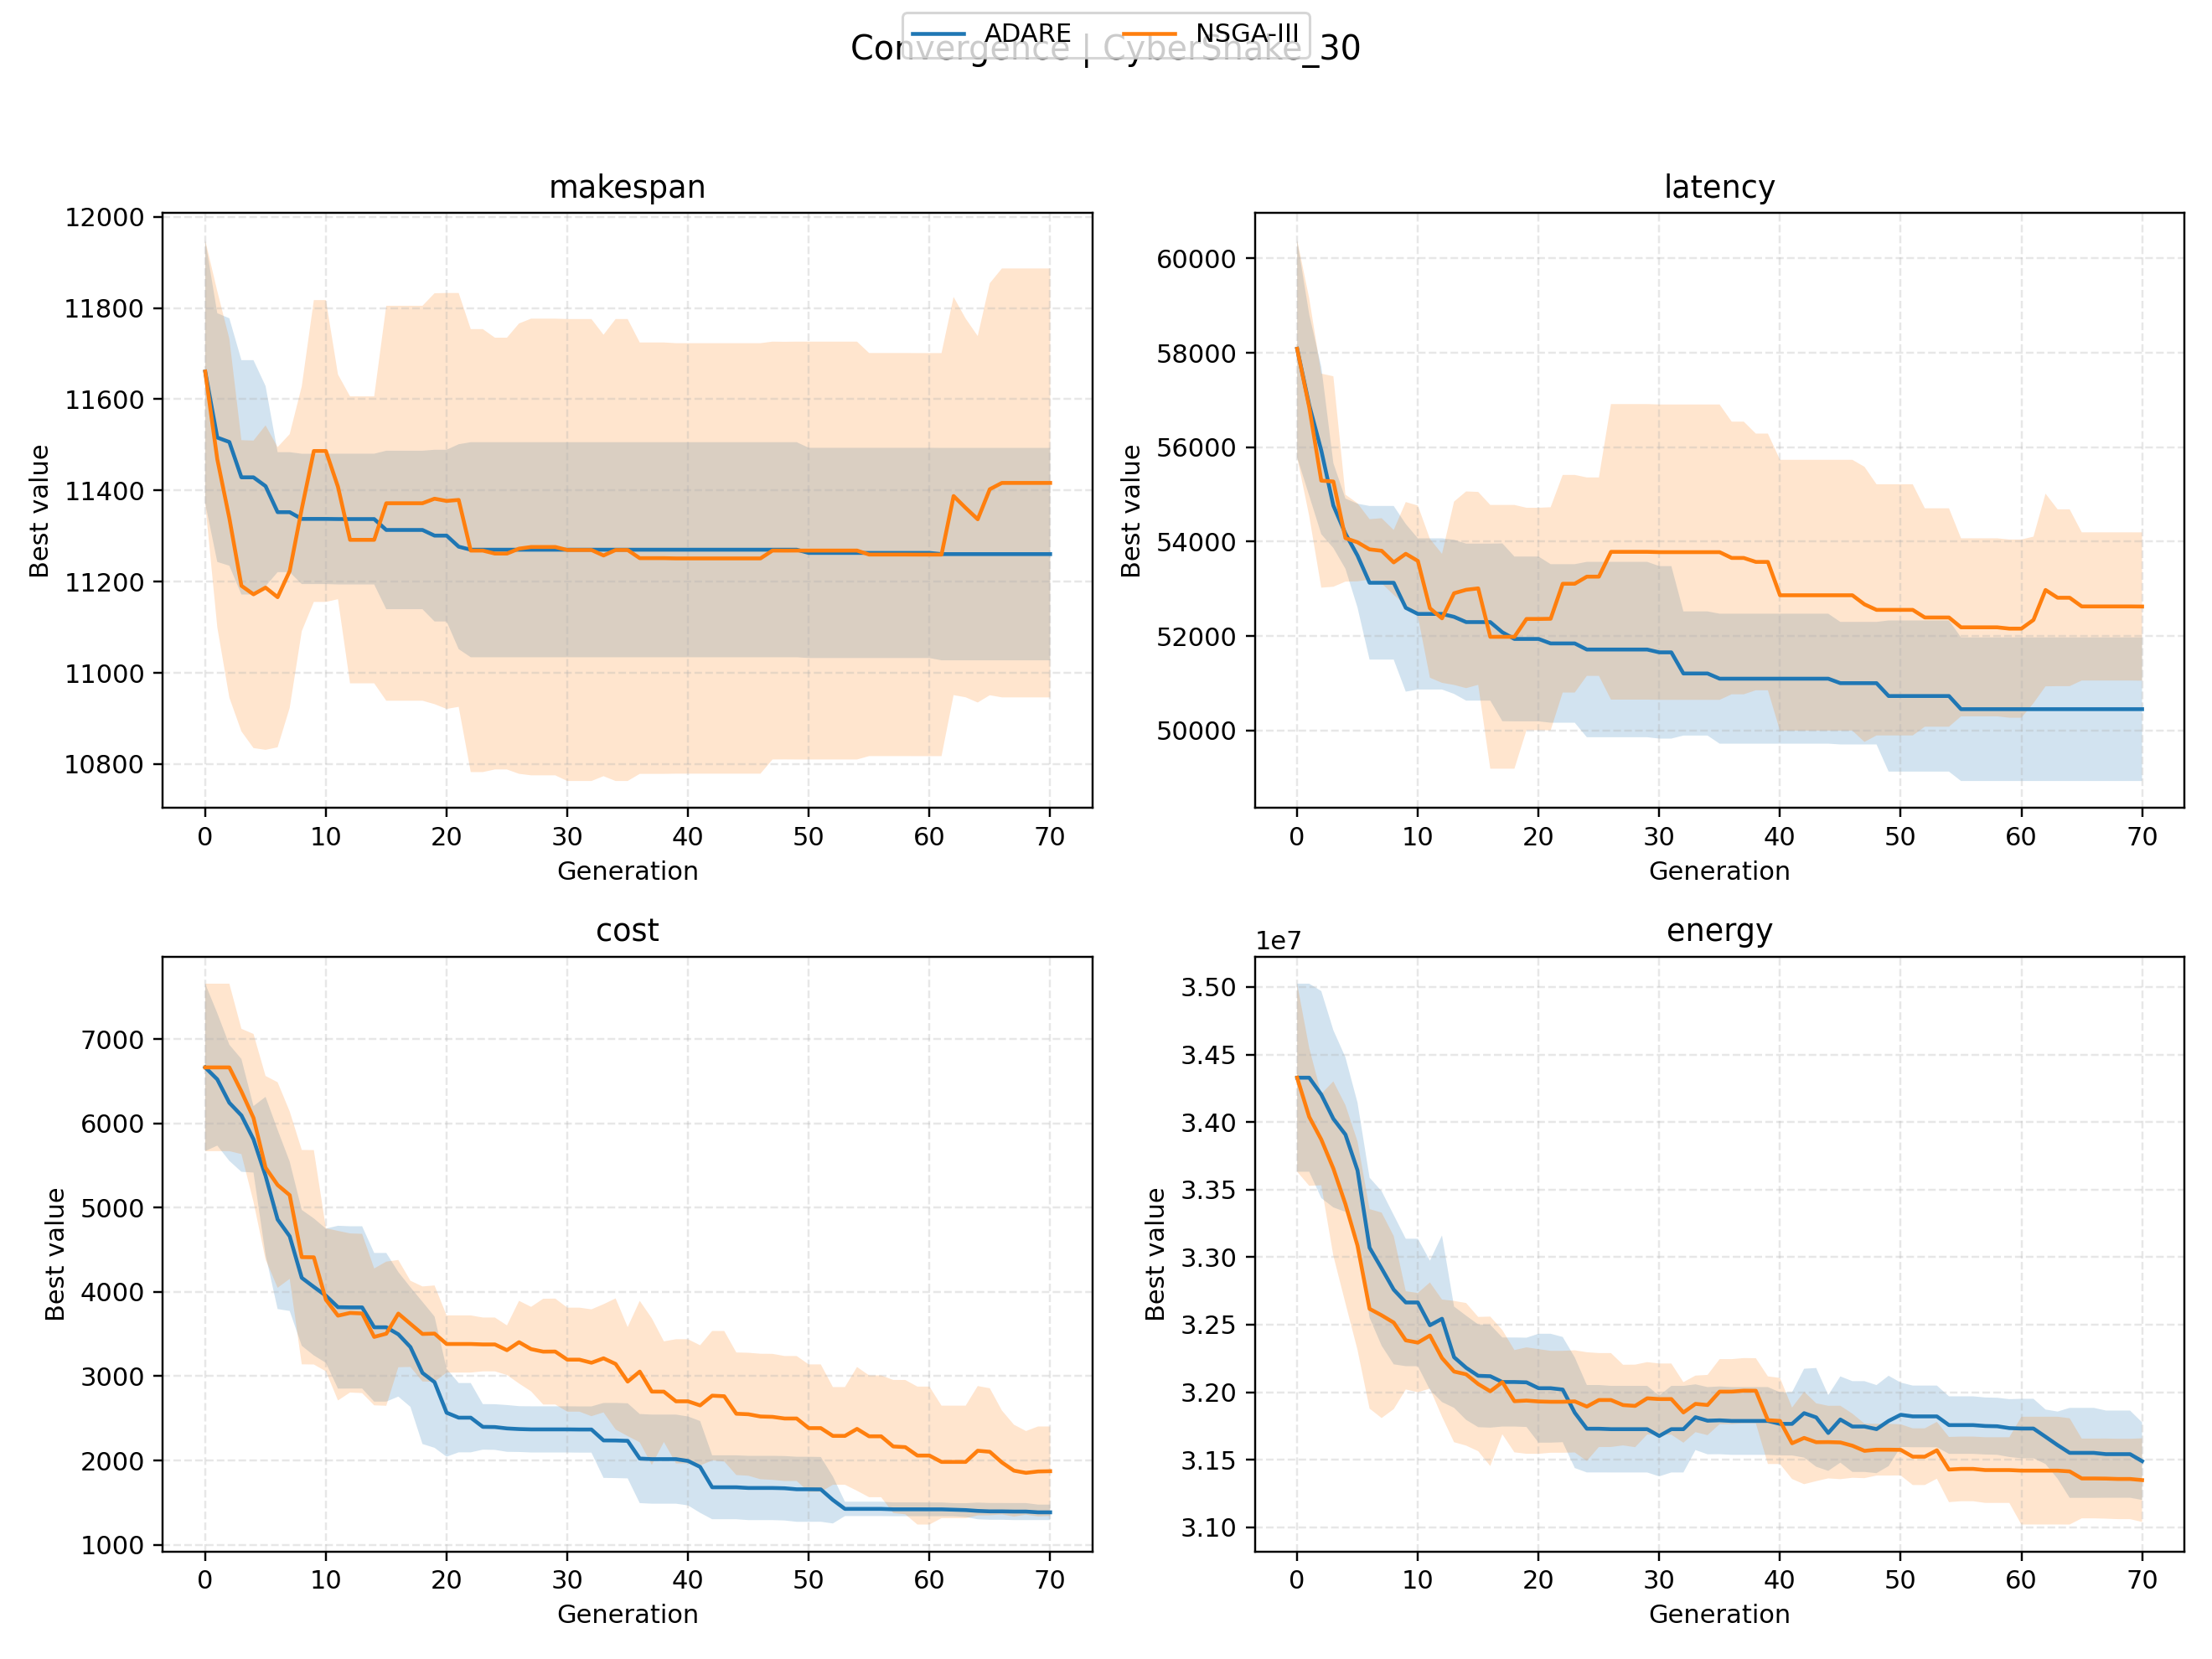
\includegraphics[width=\linewidth]{convergence_test_cybershake30.png}\\[-0.5ex]
\scriptsize (b) CyberShake\_30
\end{minipage}

\vspace{0.6ex}

\begin{minipage}[t]{0.68\textwidth}
\centering
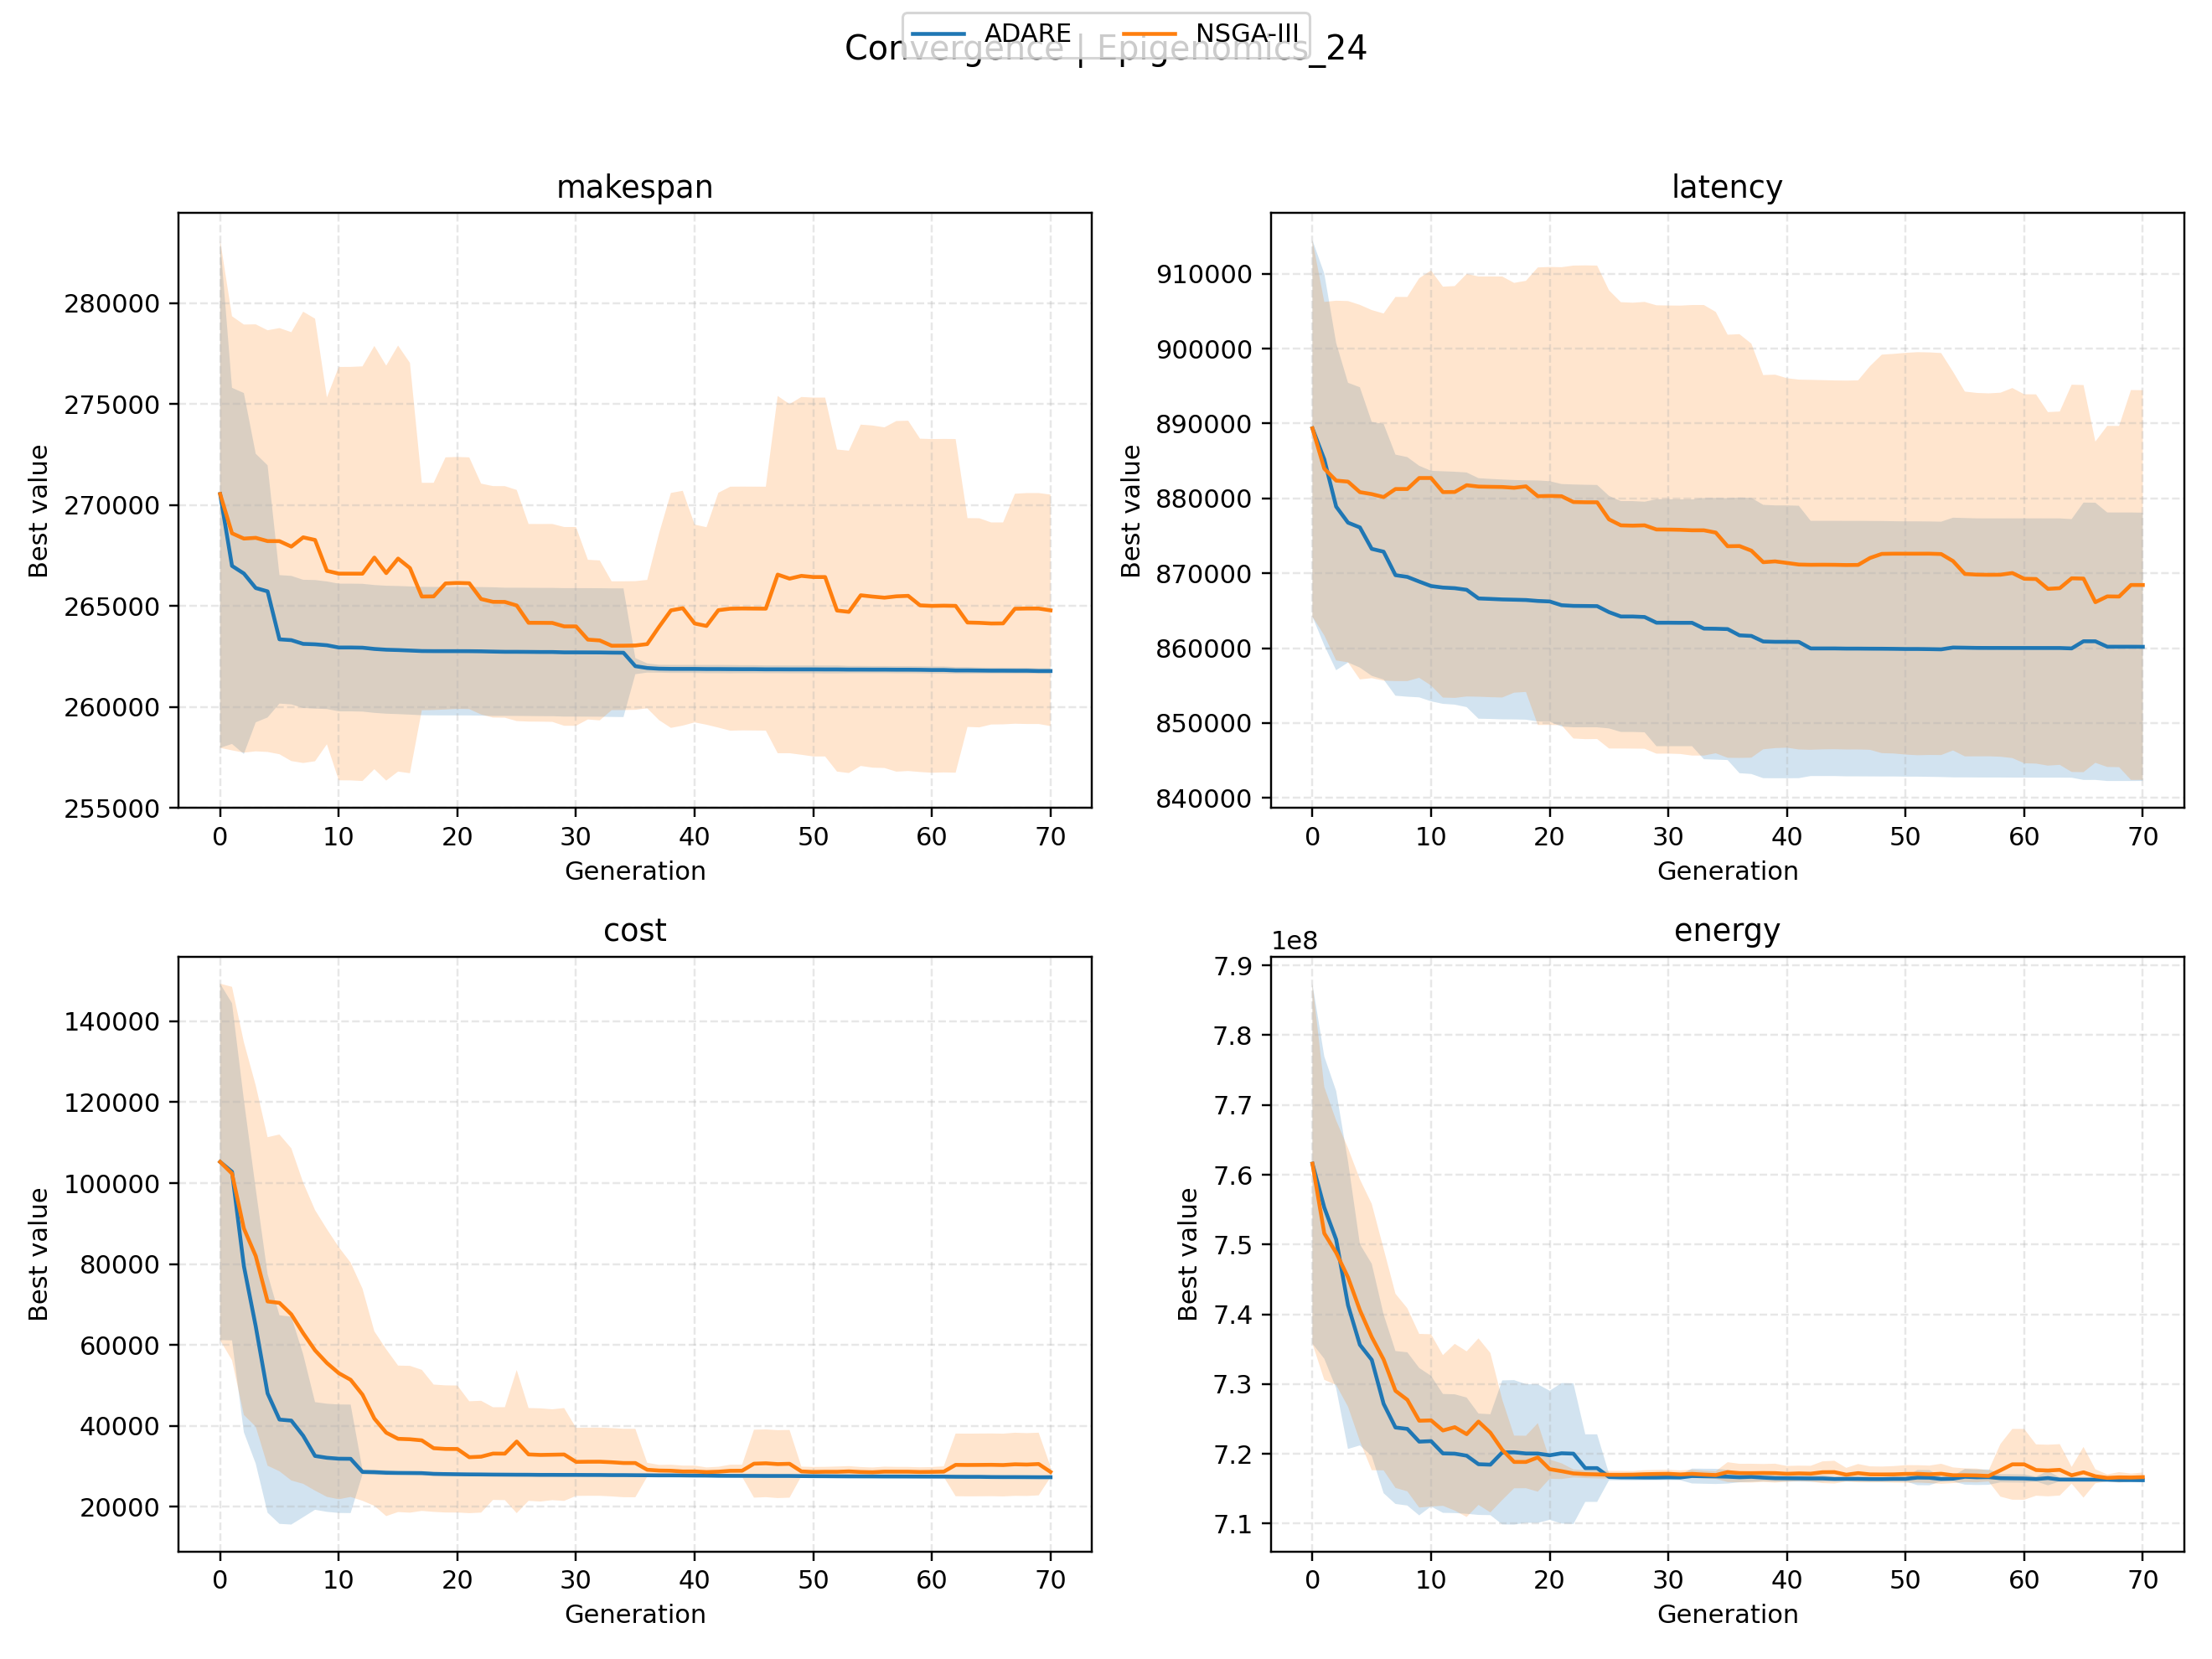
\includegraphics[width=\linewidth]{convergence_test_epigenomics24.png}\\[-0.5ex]
\scriptsize (c) Epigenomics\_24
\end{minipage}
\caption{Convergence traces (best objective values by generation) for Montage, CyberShake, and Epigenomics. Larger panels are used to improve readability of generation-wise trajectories and confidence bands.}
\label{fig:conv_all}
\end{figure}

Figure~\ref{fig:conv_all} makes the control effect visible in our runs. This matters. We see earlier trajectory separation on Montage and CyberShake, and later generations stabilize differently. Epigenomics still improves, mainly through front structure, while runtime movement stays smaller.

% Discussion refinement
At this point, the practical question is less ``does ADARE ever help?'' and more ``when does the adaptive layer help most, and where are its limits?'' The discussion below addresses that question directly.
\section{Discussion}
\subsection{Why Static NSGA-III Underperforms in Heterogeneous Environments}
% Discussion refinement
In our setting, the main weakness of a static NSGA-III pipeline is not the selection operator itself; NSGA-III's reference-point mechanism remains a strong many-objective baseline. The recurring issue is \emph{operator control rigidity}. Fixed crossover and mutation schedules assume a reward landscape that stays roughly stable, but workflow scheduling across heterogeneous edge, fog, and cloud resources shows phase changes during search.

Early generations benefit from broad exploration to discover useful task-node assignments under precedence and bandwidth constraints. Later generations benefit more from operators that preserve partial structure and refine local trade-offs. A static schedule cannot represent this shift explicitly, while ADARE's controller adapts operator preference from observed rewards. The convergence plots were useful here because they exposed this phase dependence before the aggregate statistics made it obvious.
\subsection{Justification of Experimental Choices}
\paragraph{Population size and generation count.}
We use population size 100 and 70 generations to keep comparisons computationally affordable on a local workstation while preserving enough diversity for four-objective optimization. Increasing population size improves front coverage but raises evaluator cost in practice through more offspring evaluations and more frequent archive maintenance. The chosen configuration is a compromise between statistical replication and per-run search depth.

\paragraph{Seeding and fairness.}
Seed control is not a cosmetic choice. In stochastic MOEAs, comparing unmatched runs can confound algorithmic differences with initialization variance. Our paired design uses the same initial population for ADARE and NSGA-III for every run, which makes Wilcoxon and Cliff's delta more informative.

\paragraph{Why 20 runs.}
The original artifact analysis used 6 runs. In our runs, that count exposed strong effects but remained fragile for smaller effect-size comparisons, especially runtime relative to HV/IGD/spacing gains. We moved to 20 paired runs to stabilize mean estimates and effect sizes. Table~\ref{tab:stats20} shows that directions remain favorable while effect sizes still vary by benchmark and metric.

\subsection{Sensitivity and Robustness Trends}
Our observations suggest three sensitivity patterns.
\begin{enumerate}
    \item \textbf{Run count sensitivity}: metrics with smaller effect sizes (most clearly runtime on Epigenomics in our final protocol) are sensitive to the number of repetitions and should not be interpreted from very small samples.
    \item \textbf{Mutation/Archive sensitivity}: ADARE's strongest empirical gains are associated with spacing, coverage, and objective extremes, indicating that density-aware mutation and archive guidance dominate the observed improvements in difficult landscapes.
    \item \textbf{Benchmark dependence}: ADARE delivers strong quality gains on all three workflows, but quality and runtime do not move with the same amplitude on every instance. Epigenomics shows a smaller runtime effect size than CyberShake or Montage despite clear quality improvements.
\end{enumerate}

These patterns support the adaptive-control interpretation in our runs. Under the reported 20-run protocol, ADARE is superior on all tracked quality metrics, yet the \emph{magnitude} of improvement still depends on benchmark structure. For that reason, we avoid benchmark-independent effect-size claims from smaller repetition counts, even when win/loss counts look unambiguous.
\subsection{Limitations and Artifact Scope}
% Discussion refinement
Two limitations should be stated explicitly. First, the current artifact directly implements NSGA-III as the paired baseline; NSGA-II and MOEA/D are included in our comparative positioning but not yet re-implemented under the same evaluator in this code snapshot. Second, while we provide the required V1--V5 ablation protocol and variant mapping, the full 20-run ablation sweep is deferred to a dedicated artifact extension because it substantially expands total runtime on a local workstation.

These limitations do not invalidate the main ADARE-vs-NSGA-III comparison, but they narrow the scope of what can be concluded from this version of the artifact. In particular, the broader baseline and ablation story is a reproducibility/engineering completion task rather than a theoretical gap.
\section{Conclusion}
% Discussion refinement
We reframed ADARE as an online control layer for many-objective workflow scheduling rather than as a simple scheduler variant. This framing is technically useful because it explains why operator-level learning is central to the method, while the evolutionary backbone can remain largely unchanged.

Under a fairness-controlled protocol (same initialization, same budget, same evaluator) and a stronger statistical setup (20 paired runs per benchmark), ADARE improves overall many-objective search quality and runtime against NSGA-III on three heterogeneous workflow instances. In our runs, gains are strongest in HV, coverage, spacing, and objective extremes, and CyberShake shows the clearest combined benefit. Runtime also improves on all three benchmarks in the final protocol, although the Epigenomics runtime effect remains smaller than its quality effects. Measured control overhead stays near 5\% on average, preserving practical usability on a local workstation.

For the ECML PKDD framing, the main takeaway is that workflow scheduling in heterogeneous distributed systems benefits from treating evolutionary operator choice as an \emph{online learning control problem}. Future work will complete the 20-run V1--V5 ablation sweep and extend the artifact with directly implemented NSGA-II and MOEA/D baselines under the same evaluator.
\enlargethispage{3\baselineskip}
% Author reasoning clarification
\begin{thebibliography}{99}
\footnotesize
\setlength{\itemsep}{0pt}
\setlength{\parskip}{0pt}
\setlength{\parsep}{0pt}
\bibitem{topcuoglu2002heft}
Topcuoglu, H., Hariri, S., Wu, M.-Y.: Performance-effective and low-complexity task scheduling for heterogeneous computing. IEEE Transactions on Parallel and Distributed Systems \textbf{13}(3), 260--274 (2002)

\bibitem{bonomi2012fog}
Bonomi, F., Milito, R., Zhu, J., Addepalli, S.: Fog computing and its role in the Internet of Things. In: MCC Workshop on Mobile Cloud Computing, pp.~13--16 (2012)

\bibitem{deb2002nsga2}
Deb, K., Pratap, A., Agarwal, S., Meyarivan, T.: A fast and elitist multiobjective genetic algorithm: NSGA-II. IEEE Transactions on Evolutionary Computation \textbf{6}(2), 182--197 (2002)

\bibitem{zhang2007moead}
Zhang, Q., Li, H.: MOEA/D: A multiobjective evolutionary algorithm based on decomposition. IEEE Transactions on Evolutionary Computation \textbf{11}(6), 712--731 (2007)

\bibitem{coleman2021wfcommons}
Coleman, T., Babuji, Y., Li, H., et al.: WfCommons: A framework for enabling scientific workflow research and development. Scientific Data \textbf{9}, 220 (2022).

\bibitem{deb2014nsga3}
Deb, K., Jain, H.: An evolutionary many-objective optimization algorithm using reference-point-based nondominated sorting approach, part I: Solving problems with box constraints. IEEE Transactions on Evolutionary Computation \textbf{18}(4), 577--601 (2014)

\bibitem{auer2002ucb}
Auer, P., Cesa-Bianchi, N., Fischer, P.: Finite-time analysis of the multiarmed bandit problem. Machine Learning \textbf{47}, 235--256 (2002)

\bibitem{besbes2014nonstationary}
Besbes, O., Gur, Y., Zeevi, A.: Stochastic multi-armed-bandit problem with non-stationary rewards. In: Advances in Neural Information Processing Systems (NeurIPS), vol.~27 (2014)

\bibitem{jiao2023ovea}
Jiao, K., Chen, J., Xin, B., Li, L.: OVEA: A reference vector based multiobjective evolutionary algorithm with Q-learning for operator adaptation. Evolutionary Computation \textbf{31}(3), 375--400 (2023)

\bibitem{song2024survey}
Song, A., Wang, J., Li, K., Zhang, Q.: Reinforcement learning-assisted evolutionary algorithm: A survey and research opportunities. ACM Computing Surveys \textbf{56}(12), Article 311 (2024)

\bibitem{wang2025mrlmoea}
Wang, K., Wang, Y., Xie, X., Yu, S., Zhang, Q.: MRL-MOEA: Multi-role learning based many-objective evolutionary algorithm. Scientific Reports \textbf{15}, 25039 (2025)

\bibitem{xue2025qlmoead}
Xue, J., Yang, S., Zhao, X., Hu, Y.: QLMOEA/D-AWA: A Q-learning-based decomposition multi-objective optimization evolutionary algorithm with adaptive weight adjustment. Scientific Reports \textbf{15}, 17290 (2025)

\bibitem{cui2026drlmmea}
Cui, W., Song, A., Wang, J., Zhang, Q.: DRLMMEA: Deep reinforcement learning-assisted many-objective evolutionary algorithm. Nature Communications \textbf{17}, 1084 (2026)

\bibitem{mao2017mecsurvey}
Mao, Y., You, C., Zhang, J., Huang, K., Letaief, K.B.: A survey on mobile edge computing: The communication perspective. IEEE Communications Surveys \& Tutorials \textbf{19}(4), 2322--2358 (2017)

\bibitem{wilcoxon1945}
Wilcoxon, F.: Individual comparisons by ranking methods. Biometrics Bulletin \textbf{1}(6), 80--83 (1945)

\bibitem{cliff1993}
Cliff, N.: Dominance statistics: Ordinal analyses to answer ordinal questions. Psychological Bulletin \textbf{114}(3), 494--509 (1993)

\bibitem{karafotias2015parameter}
Karafotias, G., Hoogendoorn, M., Eiben, A.E.: Parameter control in evolutionary algorithms: Trends and challenges. IEEE Transactions on Evolutionary Computation \textbf{19}(2), 167--187 (2015)

\bibitem{coello2007emo}
Coello Coello, C.A., Lamont, G.B., Van Veldhuizen, D.A.: Evolutionary Algorithms for Solving Multi-Objective Problems, 2nd edn. Springer (2007)

\bibitem{pegasus}
Deelman, E., Singh, G., Su, M.-H., et al.: Pegasus: A framework for mapping complex scientific workflows onto distributed systems. Scientific Programming \textbf{13}(3), 219--237 (2005)

\bibitem{wfcommonsrepo}
WfCommons Project: WfCommons: benchmark instances and workflow tools. \url{https://wfcommons.org/} (accessed February 24, 2026)

\end{thebibliography}

\end{document}





































